\chapter{URG of generalised SIAM: RG flows and fixed point Hamiltonian}\label{siamurg}
\section{The single-impurity Anderson model}
The model is the usual single-impurity Anderson model Hamiltonian.
\begin{equation}\begin{aligned}
	\label{andham}
	\mathcal{H} = \sum_{k\sigma}\epsilon_k \hat n_{k\sigma} + \sum_{k\sigma} \left(V_{k} c^\dagger_{k\sigma} c_{d\sigma} + h.c.\right) + \epsilon_{d}\sum_\sigma  \hat n_{d\sigma} +  U \hat n_{d\uparrow} \hat n_{d\downarrow}
\end{aligned}\end{equation}
To allow the calculation of both particle and hole kinetic energies, we will write the kinetic energy part as \(\sum_{k\sigma}\epsilon_k \tau_{k\sigma}\), where \(\tau = \hat n - \frac{1}{2}\) and drop the extra constant part.
\begin{equation}
	\label{model:siam}
	\mathcal{H} = \sum_{k\sigma}\epsilon_k \tau_{k\sigma} + \sum_{k\sigma} \left(V_{k} c^\dagger_{k\sigma} c_{d\sigma} + h.c.\right) + \epsilon_{d}\sum_\sigma  \hat n_{d\sigma} +  U \hat n_{d\uparrow} \hat n_{d\downarrow}
\end{equation}
\section{Calculation of renormalisation}
The renormalisation is
\begin{equation}\begin{aligned}
\label{newh}
c^\dagger_{q\beta}T \frac{1}{\omega - H^D}T^\dagger c_{q\beta} + T^\dagger c_{q\beta}\frac{1}{\omega^\prime - H^D}c^\dagger_{q\beta}T
\end{aligned}\end{equation}
We will be decoupling an electron \(q\beta\) at the energy shell \(\epsilon_q = \pm D\). The diagonal part (that comes down in the denominator) is
\begin{equation}\begin{aligned}
	\label{term1}
H^D = \epsilon_q \tau_{q\beta} + \epsilon_{d}\hat n_{d\beta} +  U \hat n_{d\beta} \hat n_{d\bar\beta}
\end{aligned}\end{equation}
The off-diagonal part is
\begin{equation}\begin{aligned}
	c^\dagger_{q\beta}T = V_q c^\dagger_{q\beta}c_{d\beta}
\end{aligned}\end{equation}

The renormalisation from a single electron \(q\beta\) is
\begin{equation}\begin{aligned}
	\Delta H &= c^\dagger_{q\beta}c_{d\beta} \frac{1|V_q|^2}{\omega - H^D}c_{d\beta}^\dagger c_{q\beta} + c_{d\beta}^\dagger c_{q\beta}\frac{1|V_q|^2}{\omega^\prime - H^D}c^\dagger_{q\beta}c_{d\beta} \\
		 &= c^\dagger_{q\beta}c_{d\beta} \frac{|V_q|^2}{\omega - D/2 - \epsilon_d - U \hat n_{d\bar\beta}}c_{d\beta}^\dagger c_{q\beta} + c_{d\beta}^\dagger c_{q\beta}\frac{|V_q|^2}{\omega^\prime - D/2}c^\dagger_{q\beta}c_{d\beta}\\
		 &=  \frac{\hat n_{q\beta}\left( 1 - \hat n_{d\beta} \right) |V_q|^2}{\omega - D/2 - \epsilon_d - U \hat n_{d\bar\beta}} + \frac{\hat n_{d\beta}\left( 1 - \hat n_{q\beta} \right) |V_q|^2}{\omega^\prime - D/2}
\end{aligned}\end{equation}

For comparing the two \(\omega\)s, we will use the relation eq.~\ref{omegarel}: \(\omega_0^1 + \omega^1_0 = H^D_0 + H^D_1\) where \(\omega_0^1 = \omega^\prime\). \(\omega^1_0\) however is not \(\omega\). This is because the relation assumes the \(\omega\)s to be calculated at the same energy - while \(\omega^\prime\) is calculated at energy \(-D\), \(\omega\) is at energy \(D\). The \(\omega_0^1\) should hence be the \(\omega\) at energy \(-D\), which is \(-\omega\). With this in mind, the relation says
\begin{equation}\begin{aligned}
	\omega^\prime - \omega = D/2 + \epsilon_d + U \hat n_{d\beta} - D/2 
\end{aligned}\end{equation}
This gives an expression of \(\omega^\prime\) in terms of \(\omega\). Substituting this into \(\Delta H\)  gives
\begin{equation}\begin{aligned}
	\Delta H &=  \frac{\hat n_{q\beta}\left( 1 - \hat n_{d\beta} \right) |V_q|^2}{\omega - D/2 - \epsilon_d - U \hat n_{d\bar\beta}} + \frac{\hat n_{d\beta}\left( 1 - \hat n_{q\beta}\right)|V_q|^2}{\omega - D/2 +\epsilon_d + U \hat n_{d\bar\beta}}
\end{aligned}\end{equation}
The total renormalisation from the entire shell \(\pm D\) is
\begin{equation}\begin{aligned}
	\label{vanilla:siam:ren}
	\Delta H &=  \sum_{q\beta}|V_q|^2\left[\frac{\hat n_{q\beta}\left( 1 - \hat n_{d\beta} \right) }{\omega - D/2 - \epsilon_d - U \hat n_{d\bar\beta}} + \frac{\hat n_{d\beta}\left( 1 - \hat n_{q\beta}\right)}{\omega - D/2 +\epsilon_d + U \hat n_{d\bar\beta}}\right] \\
		 &= \sum_q |V_q|^2 \left[\frac{\left(1 - \hat n_{d\beta}\right)\hat n_{d\overline\beta}}{\omega - \frac{1}{2}\epsilon_q - \epsilon_d - U} + \frac{\left(1 - \hat n_{d\beta}\right)\left( 1-\hat n_{d\overline\beta} \right)}{\omega - \frac{1}{2}\epsilon_q - \epsilon_d} + \frac{\hat n_{d\beta} \hat n_{d\overline\beta}}{\omega - \frac{1}{2}\epsilon_q + \epsilon_d + U} + \frac{\hat n_{d\beta}\left( 1- \hat n_{d\overline\beta}\right) }{\omega - \frac{1}{2}\epsilon_q + \epsilon_d}\right]
\end{aligned}\end{equation}
\section{Scaling equations for the SIAM}
Once we have the renormalisation for decoupling one electronic or hole state, we can just sum over the spins and momenta to get the total renormalisation upon decoupling the entire shells \(\pm \epsilon_q\). From the structure of \(\Delta \mathcal{H}\) in eq.~\ref{vanilla:siam:ren}, we can see that there are renormalisations to all three configuration energies of the impurity: the doublon energy \(E_2\) corresponding to the state  \(\hat n_{d\beta}\hat n_{d\overline\beta}\), the single energy \(E_1\) corresponding to (\(\hat n_{d\beta}(1 - \hat n_{d\overline\beta}) + \hat n_{d\overline\beta}(1 - \hat n_{d\beta})\), and the holon energy \(E_0\) corresponding to \((1 - \hat n_{d\beta})(1 - \hat n_{d\overline\beta}) + \hat n_{d\overline\beta}(1 - \hat n_{d\beta})\).
\begin{equation}\begin{aligned}
	\label{urg-siam}
	\Delta E_2 &= +2\sum_{q}\frac{|V_q|^2}{\omega - \frac{1}{2}\epsilon_q + \epsilon_d + U }\\
	\Delta E_1 &= +\sum_{q}\frac{|V_q|^2}{\omega - \frac{1}{2}\epsilon_q + \epsilon_d} + \sum_{q}\frac{|V_q|^2}{\omega - \frac{1}{2}\epsilon_q - \epsilon_d - U}\\
	\Delta E_0 &= +2\sum_{q}\frac{|V_q|^2}{\omega - \frac{1}{2}\epsilon_q - \epsilon_d}
\end{aligned}\end{equation}
Using the relations \(\epsilon_d = E_1 - E_0\) and \(U = E_2 + E_0 - 2E_1\), we can write
\begin{equation}\begin{aligned}
	\Delta \epsilon_d &= +\sum_{q}\frac{|V_q|^2}{\omega - \frac{1}{2}\epsilon_q + \epsilon_d} + \sum_{q}\frac{|V_q|^2}{\omega - \frac{1}{2}\epsilon_q - \epsilon_d - U} - 2\sum_{q}\frac{|V_q|^2}{\omega - \frac{1}{2}\epsilon_q - \epsilon_d}\\
	\Delta U &= \sum_{q}\frac{2|V_q|^2}{\omega - \frac{1}{2}\epsilon_q + \epsilon_d + U } + \sum_{q}\frac{2|V_q|^2}{\omega - \frac{1}{2}\epsilon_q - \epsilon_d} - \sum_{q}\frac{2|V_q|^2}{\omega - \frac{1}{2}\epsilon_q + \epsilon_d} - \sum_{q}\frac{2|V_q|^2}{\omega - \frac{1}{2}\epsilon_q - \epsilon_d - U}\\
\end{aligned}\end{equation}
\section{Connection to poor man's scaling}\label{urg2pms}
To obtain the results of Poor Man's scaling \cite{haldane}\cite{Jefferson},  we can look at various regimes. First we look at the case when both \(\epsilon_d\) and \(U\) are small such that both the singly-occupied and doubly-occupied subspaces of the impurity are comfortably inside the bandwidth, \(U,\epsilon_d \ll \epsilon_q\). We can then ignore the \(\epsilon_d\) and \(U\) in the denominator compared to the \(\epsilon_q\).
\begin{equation}\begin{aligned}
\Delta \epsilon_d &= \sum_{q}\frac{|V_q|^2}{\omega - \frac{1}{2}\epsilon_q} + \sum_{q}\frac{|V_q|^2}{\omega - \frac{1}{2}\epsilon_q} - 2\sum_{q}\frac{|V_q|^2}{\omega - \frac{1}{2}\epsilon_q}\\
\Delta U &= 2\sum_{q}\frac{|V_q|^2}{\omega - \frac{1}{2}\epsilon_q} + 2\sum_{q}\frac{|V_q|^2}{\omega - \frac{1}{2}\epsilon_q} - 2\sum_{q}\frac{|V_q|^2}{\omega - \frac{1}{2}\epsilon_q} - 2\sum_{q}\frac{|V_q|^2}{\omega - \frac{1}{2}\epsilon_q}
\end{aligned}\end{equation}
Assuming the upper and lower band edges are symmetrical such that \(\sum_{-D} = \sum_D\), we get \(\Delta \epsilon_d = \Delta U = 0\). 

In the regime \(U \gg \epsilon_q \gg \epsilon_d\), the doubly-occupied state is far above the bandwidth. We can now ignore the terms that have \(U\) in the denominator. We get
\begin{equation}\begin{aligned}
\Delta \epsilon_d &= \sum_{q}\frac{|V_q|^2}{\omega - \frac{1}{2}\epsilon_q} - 2\sum_{q}\frac{|V_q|^2}{\omega - \frac{1}{2}\epsilon_q}\\
\Delta U &= 2\sum_{q}\frac{|V_q|^2}{\omega - \frac{1}{2}\epsilon_q}  - 2\sum_{q}\frac{|V_q|^2}{\omega - \frac{1}{2}\epsilon_q} 
\end{aligned}\end{equation}
Again assuming symmetrical upper and lower edges, and isotropic dispersion \(\epsilon_q=D\) and \(\sum_q |V|^2 = \frac{\Delta}{\pi}|\delta D|\), we get
\begin{equation}\begin{aligned}
\Delta U &= 0\\
\delta \epsilon_d &= -\frac{\Delta}{\pi}\frac{1}{\omega - \frac{1}{2} D}
\end{aligned}\end{equation}
There we replaced the difference symbol \(\Delta\) with \(\delta\) to avoid confusion with the hybridisation \(\Delta \sim \sum V^2\). For low quantum fluctuations, we can ignore the renormalisation in the couplings and replace \(\omega\) with the initial conduction electron energy: \(\omega = \epsilon_q\tau_{q\beta} = -\frac{1}{2} D\).
\begin{equation}\begin{aligned}
\delta \epsilon_d &= \frac{\Delta}{\pi}\frac{\delta D}{D}
\end{aligned}\end{equation}
This is the one-loop scaling equation.
\section{Preservation of particle-hole symmetry}
The Anderson model Hamiltonian, eq.~\ref{andham}, has an impurity particle-hole symmetry for a certain condition of the couplings. To see this, we apply the particle-hole transformation \(c_k \to c^\dagger_k, c_d \to -c^\dagger_d\) to the Hamiltonian. Since we are looking at the impurity symmetry, we will only look at the terms involving the impurity. The particle-hole symmetry of the conduction bath is a separate thing and that requires a specific lattice. Hence we will not consider kinetic energy term in this discussion. The rest of the terms transform as
\begin{gather}
    \epsilon_d \sum_\sigma \hat n_{d\sigma} \to 2\epsilon_d - \epsilon_d \sum_\sigma \hat n_{d\sigma}\label{imp1}\\
U \hat n_{d\uparrow}\hat n_{d\downarrow} \to U \hat n_{d\uparrow}\hat n_{d\downarrow} - U\sum_\sigma \hat n_{d\sigma} + U\label{imp2}\\
\sum_{k\sigma}V(k)c^\dagger_{k\sigma}c_{d\sigma} + hc \to \sum_{k\sigma}-V(k)c_{k\sigma}c^\dagger_{d\sigma} + hc = \sum_{k\sigma}V^*(k)c^\dagger_{k\sigma}c_{d\sigma} + hc \label{hop}
\end{gather}
The impurity-bath hopping term can be made symmetric by making \(V(k)\) real; we would then have, from eq.~\ref{hop},
\begin{equation}\begin{aligned}
	V(k)\left(c^\dagger_{k\sigma}c_{d\sigma} + c^\dagger_{d\sigma}c_{k\sigma}\right)\to V(k)\left(c^\dagger_{d\sigma}c_{k\sigma} + c^\dagger_{k\sigma}c_{d\sigma}\right)
\end{aligned}\end{equation}
The impurity diagonal terms, \(\epsilon_d\) and \(U\), require a specific condition. Combining eqs.~\ref{imp1} and \ref{imp2},
\begin{equation}\begin{aligned}
	\epsilon_d\hat n_{d\sigma} + U\hat n_{d\uparrow}\hat n_{d\downarrow} \to \left(-\epsilon_d - U\right)\hat n_{d\sigma} + U\hat n_{d\uparrow}\hat n_{d\downarrow}
\end{aligned}\end{equation}
We dropped some constant terms in the transformed Hamiltonian. For particle-hole symmetry, the left and right hand sides must be same. The required condition is thus 
\begin{equation}\begin{aligned}
	\label{phs}
\epsilon_d = -\epsilon_d - U \implies \epsilon_d + \frac{1}{2} U = 0
\end{aligned}\end{equation}
\begin{minipage}{0.5\textwidth}
    This same condition can be obtained in a more physical way. If we consider the singly-occupied state of the impurity as the reference state, the doubly-occupied state is the particle-excitation and the vacant state is the hole excitation. The energy of this particle state is \(E_2 = 2\epsilon_d + U\) and that of the hole state is \(E_0 = 0\). Particle-hole symmetry then requires the particle and hole levels to be degenerate, which means \(E_2 = E_0\), and we recover the condition eq.~\ref{phs}.
\end{minipage}
\hfill
\begin{minipage}{0.4\textwidth}
    \centering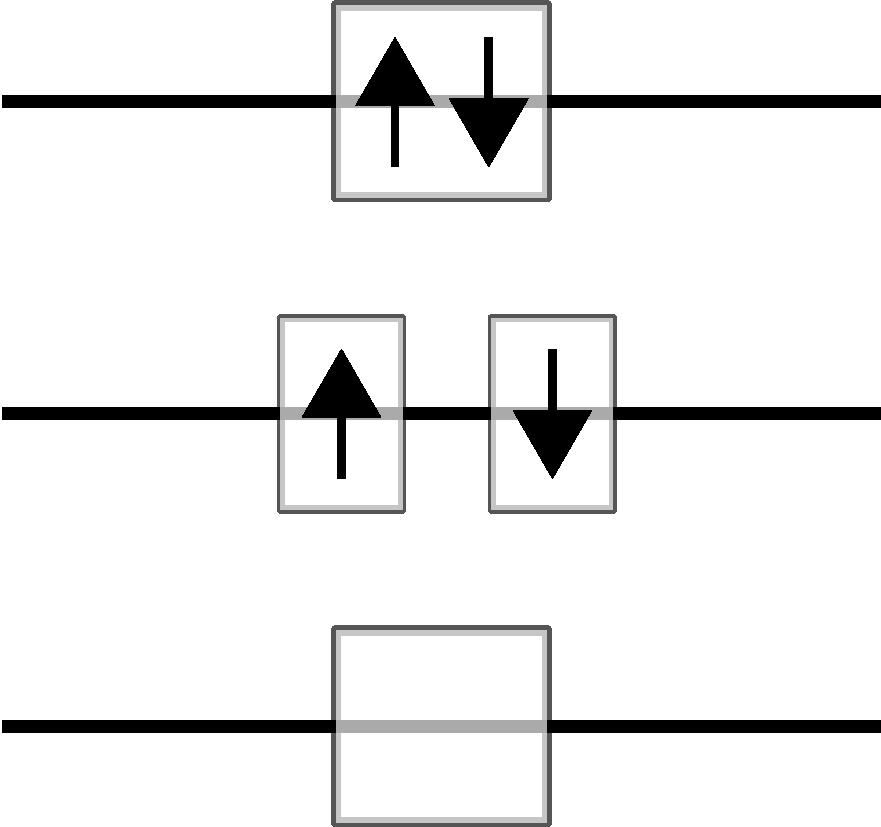
\includegraphics[width=0.8\textwidth]{phsymm.pdf}
    \captionof{figure}{Particle and hole excitations of the impurity}
\end{minipage}

Since the URG is unitary, if we start from a model that is particle-hole symmetric, the RG equations should uphold that symmetry. What this means is that if we have \(\epsilon_d + \frac{1}{2} U = 0\) in the bare model, the new couplings should also satisfy \(\epsilon_d^\prime + \frac{1}{2} U^\prime = 0\). This means we must have 
\begin{equation}\begin{aligned}
	\Delta\left(\epsilon_d + \frac{1}{2} U\right) = 0
\end{aligned}\end{equation}
The quantity \(\gamma = \epsilon_d + \frac{1}{2} U\) is thus an RG-invariant for the particle-hole symmetric model; it does not change under the RG flow. It is often referred to as the asymmetry parameter; it quantifies the asymmetry in the model. We need to check if our equations satisfy this. Looking at the RG equations for \(\epsilon_d\) and \(U\), we can find the RG equation for the asymmetry parameter. The slightly easier way is to just note that the renormalisation in \(E_2\) should be equal to the renormalisation in \(E_0\), in order for p-h symmetry to hold.
\begin{equation}\begin{aligned}
\Delta E_2 &= 2 \frac{\Delta}{\pi}\frac{1}{\omega - D + \epsilon_d + U}, \Delta E_0 &= 2 \frac{\Delta}{\pi}\frac{1}{\omega - D - \epsilon_d}
\end{aligned}\end{equation}
If we start with a particle-hole symmetric model, we will have \(-\epsilon_d = \epsilon_d + U\). Substituting that gives \(\Delta E_2= \Delta E_0\). This shows that the doublon and holon states remain equidistant from the single-particle level, thus maintaining particle-hole symmetry along the flow.
\section{Numerical analysis of the particle-hole symmetric RG equations}
We will specialize to the particle-hole symmetric case, \(2\epsilon_d + U = 0\), and a symmetric energy shell \(\epsilon_q = D\), and look at the scaling behavior of \(\epsilon_d\).
\begin{equation}\begin{aligned}
	\Delta \epsilon_d = -4|V|^2 \frac{\epsilon_d}{\left( \omega - \frac{1}{2}D \right)^2 - \epsilon_d^2}
\end{aligned}\end{equation}
Since the equation is symmetric under \(\epsilon_d \to -\epsilon_d\), we might as well work with the magnitude of the onsite energy:
\begin{equation}\begin{aligned}
	\Delta |\epsilon_d| = -4|V|^2 \frac{|\epsilon_d|}{\left( \omega - \frac{1}{2}D \right)^2 - \epsilon_d^2}
\end{aligned}\end{equation}
Depending on the signature of the denominator, the flows will be either relevant or irrelevant.
\begin{figure}[!htpb]
	\centering
	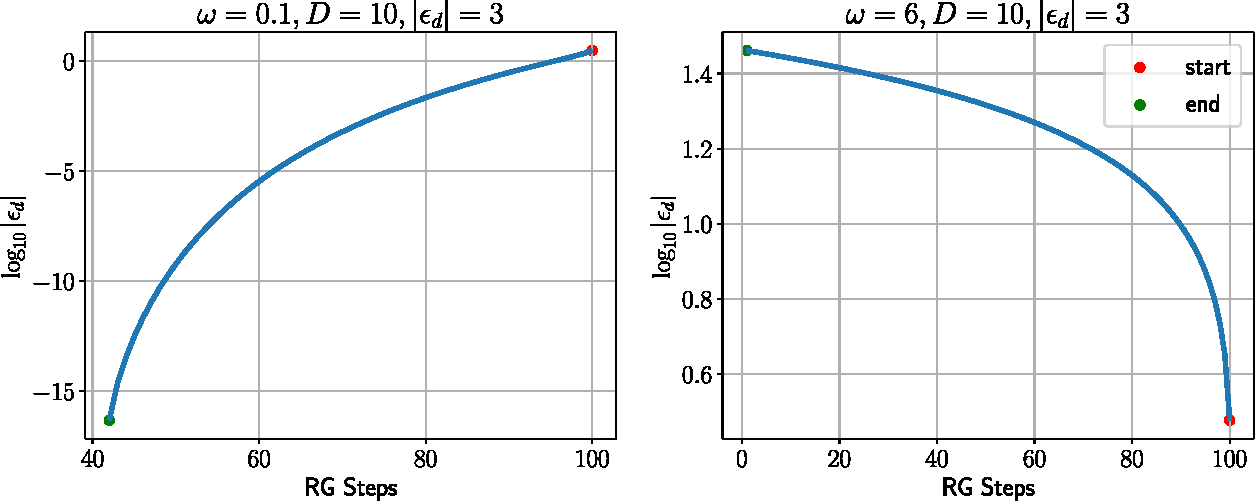
\includegraphics[width=0.99\textwidth]{../figures/ed_pure_siam.pdf}
	\caption{Left: Irrelevant flow towards \(|\epsilon_d|=0\), at low \(\omega\). Right: Relevant flow towards large \(|\epsilon_d|\), at large \(\omega\). The former can be thought of as the projection of the strong-coupling flow on to the \(\epsilon_d-D\) plane. The latter is the flow towards the local moment fixed point, if we start from a negative \(\epsilon_d\).}
\end{figure}
For the flow to the local moment fixed point, the fixed point value of \(|\epsilon_d|\) grows as we increase the bandwidth. This implies that for a thermodynamically large system, the local moment fixed point will be at \(-\epsilon_d \to \infty\). This behavior is shown in fig.~\ref{edvsD}.
\begin{figure}[htpb]
	\centering
	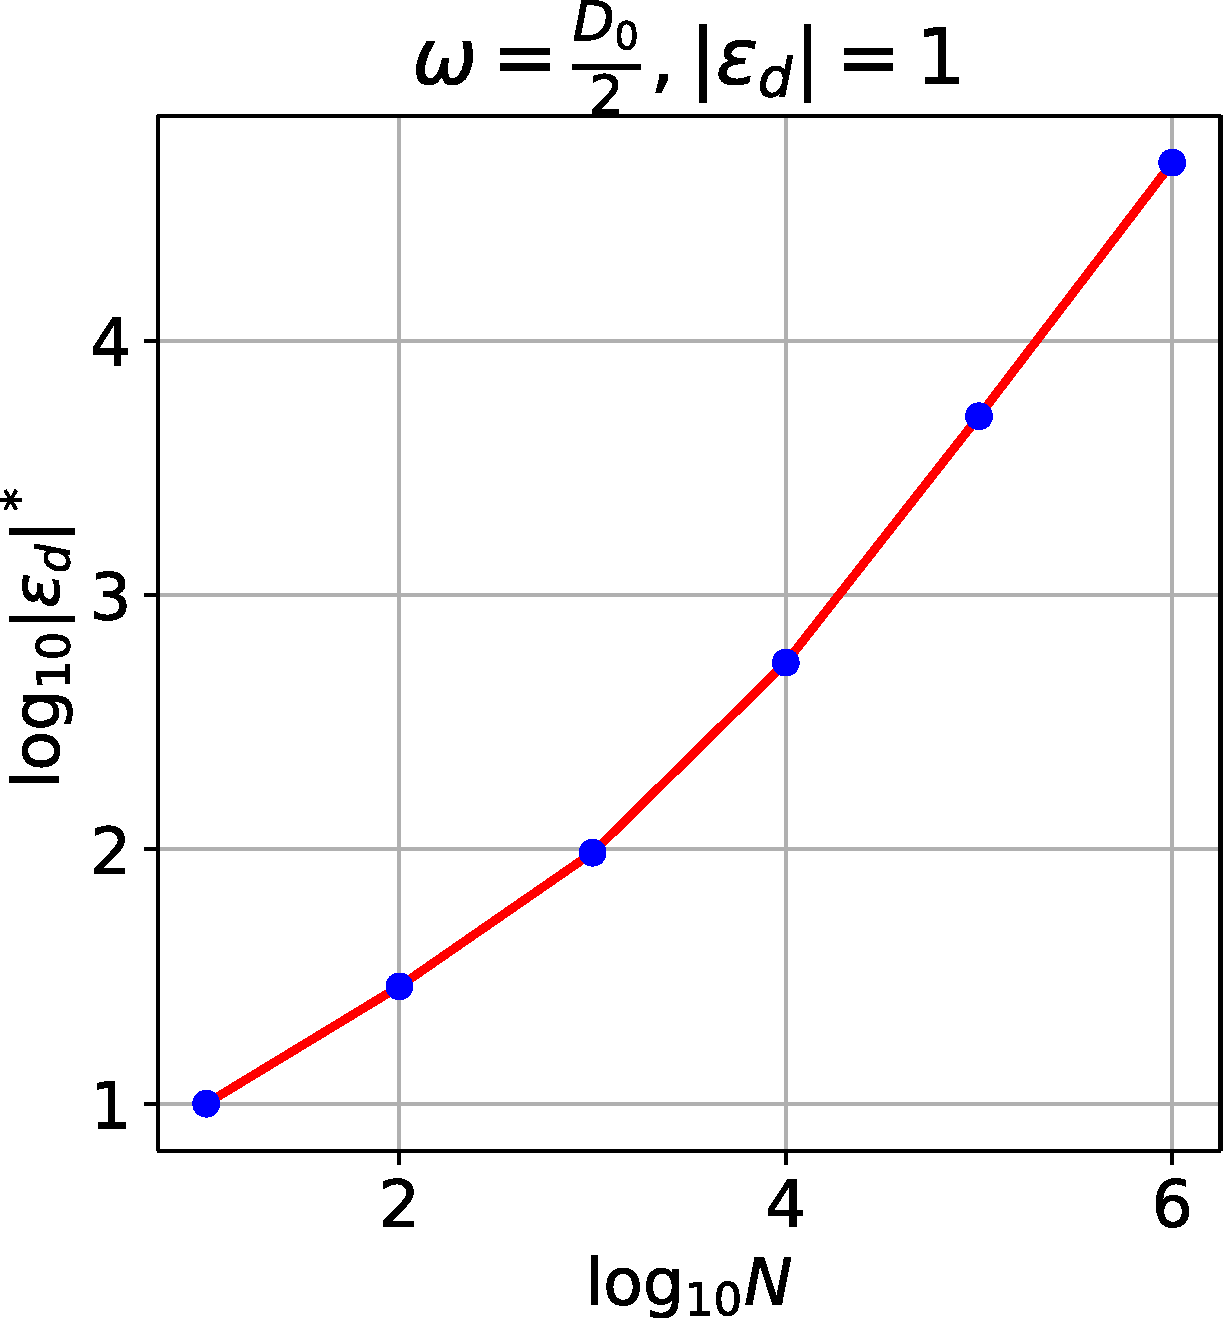
\includegraphics[width=0.6\textwidth]{../figures/ed_vs_size.pdf}
	\caption{Change in fixed point value of \(|\epsilon_d|\) with system size.}
	\label{edvsD}
\end{figure}
\section{Introduction of spin-exchange and charge isospin-exchange interactions into the SIAM: the generalised SIAM}
We will now study the generalised SIAM obtained by introducing spin-exchange and charge isospin-exchange interactions between the impurity and the conduction bath. Such terms are generated when one does a Schrieffer-Wolff transformation on the SIAM, but we will find it prudent to keep these terms in the bare model itself.

The spin-exchange interaction has the form
\begin{equation}\begin{aligned}
	J \vec{S_d}\cdot\vec{s} = J \left[S_d^z s^z + \frac{1}{2}\left( S_d^+ s^- + S_d^- s^+ \right) \right] ~,
\end{aligned}\end{equation}
where \(\vec S_d = \left(S_d^x, S_d^y, S_d^z\right) = \sum_{\alpha\beta}\vec \sigma_{\alpha\beta}c^\dagger_{d\alpha}c_{d\beta}\) is the impurity spin operator, \(\vec s = \sum_{kk^\prime\alpha\beta}\vec \sigma_{\alpha\beta}c^\dagger_{k\alpha}c_{k^\prime\beta}\) is the spin operator for the conduction bath and \(J\) is the spin-exchange coupling. The bath spin operator actually acts locally, as can be seen by Fourier transforming to real space (using the definition \(f(k) = \frac{1}{\sqrt N}\sum_r g(r)\exp(ikr)\)):
\begin{equation}\begin{aligned}
	\vec s = \sum_{k k^\prime r r^\prime} \frac{1}{N} e^{ikr - ik^\prime r^\prime} \vec \sigma_{\alpha\beta} c^\dagger_{r\alpha} c_{r^\prime\beta} = \sum_{rr^\prime}\frac{1}{N}\vec \sigma_{\alpha\beta} c^\dagger_{r\alpha} c_{r^\prime\beta} N \delta(r)\delta(r^\prime) = \vec \sigma_{\alpha\beta} c^\dagger_{0\alpha} c_{0\beta}
\end{aligned}\end{equation}

In order to introduce the charge isospin coupling, we define the Nambu spinor \cite{nambu,anderson_superc} \(\psi^k = \left( c_{k\uparrow} \quad c^\dagger_{k\downarrow} \right)\), and the charge isospin \cite{charge-kondo-Zitko} for the mobile conduction electrons
\begin{equation}\begin{aligned}
\vec C = \sum_{kk^\prime} {\psi^k}^\dagger \vec S \psi^{k^\prime} = \frac{1}{2}\sum_{kk^\prime\alpha\beta} {\psi^k_\alpha}^\dagger \vec \sigma_{\alpha\beta} \psi^{k^\prime}_\beta
\end{aligned}\end{equation}
The various components of the isospin are
\begin{equation}\begin{aligned}
	C^z &= \sum_{kk^\prime\sigma}\frac{1}{2} {\psi^k_\sigma}^\dagger \sigma^z_{\sigma\sigma} \psi^{k^\prime}_\sigma = \frac{1}{2}\sum_{kk^\prime\sigma}\left(c^\dagger_{k\sigma}c_{k^\prime \sigma} - \frac{1}{2}\delta_{kk^\prime}\right)\label{diagonalCz}\\
	C^x &= \sum_{kk^\prime\sigma}\frac{1}{2} {\psi^k_\sigma}^\dagger \sigma^x_{\sigma\overline\sigma} \psi^{k^\prime}_{\overline\sigma} = \sum_{kk^\prime\sigma} \frac{\sigma}{4}\left( c^\dagger_{k\sigma}c^\dagger_{k^\prime\overline\sigma} + \text{h.c.} \right) \\
	C^y &= \sum_{kk^\prime\sigma}\frac{1}{2} {\psi^k_\sigma}^\dagger \sigma^y_{\sigma\overline\sigma} \psi^{k^\prime}_{\overline\sigma} = \sum_{kk^\prime\sigma} - \frac{i\sigma}{4}\left( c^\dagger_{k\sigma}c^\dagger_{k^\prime\overline\sigma} - \text{h.c.} \right)\\
\end{aligned}\end{equation}
It is easy to verify that these operators satisfy the SU(2) commutation algebra. For example, if we write \(C^x = A + A^\dagger\) and \(C^y = B + B^\dagger\), then \(\left[ C^x, C^y \right] = \left[ A, B^\dagger \right] - \text{h.c.}\), where
\begin{equation}\begin{aligned}
	\left[ A, B^\dagger \right] = \frac{1}{4}\sum_{kk^\prime,qq^\prime}\left[ c^\dagger_{k\uparrow}c^\dagger_{k^\prime \downarrow}, i c_{q^\prime \downarrow}c_{q \uparrow} \right] = \frac{i}{4}\sum_{kq}\left(c^\dagger_{k\uparrow}c_{q \uparrow} - c_{k \downarrow}c^\dagger_{q \downarrow}\right)
\end{aligned}\end{equation}
and therefore
\begin{equation}\begin{aligned}
	\implies \left[ C^x, C^y \right] = \frac{i}{2}\sum_{kq}\left(c^\dagger_{k\uparrow}c_{q \uparrow} - c_{k \downarrow}c^\dagger_{q \downarrow}\right) = i C^z
\end{aligned}\end{equation}
There are similar operators for the impurity electron:
\begin{equation}\begin{aligned}
	\psi_d = \left( c_{d\uparrow} \quad c^\dagger_{d\downarrow}\right), &&\vec C_d = \frac{1}{2}\sum_{\beta} {\psi_{d,\alpha}}^\dagger \vec \sigma_{\alpha\beta} \psi_{d,\beta}
\end{aligned}\end{equation}
The full charge-Kondo interaction can now be written down in terms of these isospins:
\begin{equation}\begin{aligned}
	K \vec{C_d}\cdot\vec{C} = K \left[C_d^z C^z + \frac{1}{2}\left(C_d^+ C^-+ C_d^- C^+\right)\right]
\end{aligned}\end{equation}
where \(C^\pm \equiv C^x \pm iC^y\).
\begin{equation}\begin{aligned}
	C^+ = \sum_{kk^\prime} c^\dagger_{k\uparrow}c^\dagger_{k^\prime\downarrow}, && C^- = \sum_{kk^\prime}c_{k^\prime\downarrow}c_{k\uparrow}
\end{aligned}\end{equation}
The full generalised Anderson model Hamiltonian, at particle-hole symmetry, is
\begin{equation}\begin{aligned}
	\mathcal{H} = \sum_{k\sigma}\epsilon_k \tau_{k\sigma} + \epsilon_d \left( \hat n_{d \uparrow} - \hat n_{d \downarrow} \right) ^2 + \sum_{k\sigma} \left(V_{k} c^\dagger_{k\sigma} c_{d\sigma} + h.c.\right) +J \vec{S_d}\cdot\vec{s} + K \vec{C_d}\cdot\vec{C}
\end{aligned}\end{equation}

For the URG analysis, at each RG step, we decouple the electronic states \(q\beta\) on the \(k-\)space shell of radius\(\Lambda_j\). For simplicity, we will only consider those diagonal terms in the denominator that either have both \(q\beta\) and \(q\overline\beta\) or  both \(q\beta\) and \(d\) or both \(q\overline\beta\) and \(d\). Terms that have purely \(q\overline\beta\) will not be considered. Also, the scattering between just \(d\) and \(q\overline\beta\) can be ignored since it is diagonal in \(q\beta\). 
The diagonal (number-preserving) part is
\begin{equation}\begin{aligned}
	H_D = \sum_\beta\epsilon_q\tau_{q\beta} + \epsilon_d \left( \hat n_{d \uparrow} - \hat n_{d \downarrow} \right) ^2 + J S^z_ds^z_{q} + K C^z_d C^z_q\\
\end{aligned}\end{equation}
where \(s_q^z = \frac{1}{2}\left(\hat n_{q\uparrow} - \hat n_{q\downarrow}\right)\) and \(C_q^z = \frac{1}{2}\left(\hat n_{q \uparrow} + \hat n_{q \downarrow} - 1\right)\). The off-diagonal part is:
\begin{equation}\begin{aligned}
	H_X = \sum_{\beta=\uparrow,\downarrow}\left[V c^\dagger_{d\beta}c_{q\beta} + \frac{1}{2}J \sum_{k<\Lambda_N}\left\{\left(\hat n_{d \beta} - \hat n_{d \overline\beta}\right) \frac{1}{2} c^\dagger_{k\beta}c_{q\beta} + c^\dagger_{d\beta}c_{d\overline\beta}c^\dagger_{k\overline\beta}c_{q \beta}\right\} + \frac{1}{2}K \sum_{k<\Lambda_N}\left\{\left(\hat n_d -1\right)\frac{1}{2}c^\dagger_{k\beta}c_{q\beta} + \right.\right.\\
\left.\left.c^\dagger_{d\beta}c^\dagger_{d\overline\beta}c_{k\overline\beta}c_{q\beta}\right\}\right] + \text{h.c.}~.
\end{aligned}\end{equation}

\section{Calculation of renormalisation}
\subsection{Renormalisation of the impurity energy \(\epsilon_d\)}
The coupling \(\epsilon_d\) is renormalised by three kinds of vertices: \(V^2\), \(J^2\) and \(K^2\). We will consider these processes one after another. We define \(n_j\) as the number of states being decoupled on each side of the Fermi surface, at the \(j^\text{th}\) RG step. In order to treat both spin and isospin exchanges democratically, we take \(\ket{\Psi}_i = \frac{1}{2}\left(\ket{0} + \ket{q\uparrow} + \ket{q\downarrow} + \ket{q\uparrow, q\downarrow}\right) \) as the \textit{initial} state for the scattering processes. The intermediate states \(\ket{\Psi}_\text{int}\) in the particle sector \(\left(c_{q\beta}\ket{\Psi}_i\right)\) and hole sector \(\left(c^\dagger_{q\beta}\ket{\Psi}_i\right)\) will then have both spin and isospin excitations which can couple with the corresponding impurity degree of freedom. We will assume that states  \(q > k_F~\left(\epsilon_q > 0\right) \) above the Fermi surface can have only particle excitations and states below the Fermi surface can only have hole excitations. The kinetic energy part \(\epsilon_q \tau_{q\beta}\) of \(H_D\) for \(\ket{\Psi}_i\) is then zero, whereas it is always \(D/2\) for \(\ket{\Psi}_\text{int}\). To demonstrate this for a typical \(q < k_F\), the hole excitation is \(c_{q \uparrow}\ket{\Psi}_i = \frac{1}{\sqrt 2}\left(\ket{0} + \ket{q \downarrow}\right)\). This has an isospin term in the form of the \textit{holon} and a spin term in the form of the down state. Since \(\tau_{q \uparrow} = -\frac{1}{2}\) in the excited state, the kinetic energy for \(\ket{\Psi}_\text{int}\) is \(\epsilon_q \tau_{q \uparrow} = \left(-D\right)\times\left(-\frac{1}{2}\right) = D/2\).

The renormalisation arising from the first kind of terms, in the particle sector, is
\begin{equation}\begin{aligned}
	\sum_{q\beta}c^\dagger_{q\beta}c_{d\beta}\frac{V^2}{\omega - H_D}c^\dagger_{d\beta}c_{q\beta} = \sum_{q\beta}V^2 \hat n_{q\beta} \left( 1 - \hat n_{d\beta} \right)\left( \frac{1-\hat n_{d \overline\beta }}{\omega - E_0} + \frac{\hat n_{d \overline\beta}}{\omega^\prime - E_1}\right) = V^2 n_j\sum_{\beta}\left( 1 - \hat n_{d\beta} \right)\left( \frac{1-\hat n_{d \overline\beta }}{\omega_0 - E_0} + \frac{\hat n_{d \overline\beta}}{\omega_1 - E_1}\right)
\end{aligned}\end{equation}
\(q\) runs over the momentum states that are being decoupled at this RG step: \(|q| = \Lambda_j\). \(E_{1,0}\) are the diagonal parts of the Hamiltonian at \(\hat n_{d\overline \beta}=0,1\) respectively. We have \(\hat n_{d\beta}=1\) in the intermediate state because of the \(c^\dagger_{d\beta}\) in front of the Greens function. Applying \(c_{q\beta}\) on the initial state \(\ket{\Psi}_i\) leaves us with \(C^z_q = - \frac{1}{2}\) and \(s^z_q = \frac{1}{2}\overline\beta\). We also know that
\begin{equation}\begin{aligned}
	\hat n_{d\beta}=1,
	\begin{cases}
		\hat n_{d\overline\beta}=0 &\implies S_d^z = \frac{1}{2}\beta, C_d^z = 0, \epsilon_d\left(\hat n_{d\uparrow} - \hat n_{d \downarrow}\right)^2 = \epsilon_d\\	
		\hat n_{d\overline\beta}=1 &\implies S_d^z = 0, C_d^z = \frac{1}{2}, \epsilon_d\left(\hat n_{d\uparrow} - \hat n_{d \downarrow}\right)^2 = 0
	\end{cases}
\end{aligned}\end{equation}
Combining all this, we can write \(E_1 = \frac{D}{2} - \frac{K}{4}\) and \(E_0 = \frac{D}{2} + \epsilon_d - \frac{J}{4}\). In order to relate \(\omega_0\) with \(\omega_1\) with the common fluctuation scale \(\omega\) for the conduction electrons, we will replace these quantum fluctuation scales by the current renormalised values of the single-particle self-energy for the initial state from which we started scattering. For \(\hat n_{d\overline\beta}=0\), there is no additional self-energy because the impurity does not have any spin: \(\omega_0 = \omega\). For \(\hat n_{d\overline\beta} = 1\), we have an additional self-energy of \(\epsilon_d\) arising from the correlation on the impurity: \(\omega_1 = \omega + \epsilon_d\).
Substituting the values of \(E_{0,1}\) and \(\omega_{0,1}\), we get
\begin{equation}\begin{aligned}
	\label{ren_ed_Vp}
	V^2 n_j\sum_{\beta}\left( 1 - \hat n_{d\beta} \right)\left( \frac{1-\hat n_{d \overline\beta }}{\omega - \frac{D}{2} - \epsilon_d + \frac{J}{4}} + \frac{\hat n_{d \overline\beta}}{\omega - \frac{D}{2} + \epsilon_d + \frac{K}{4}}\right)
\end{aligned}\end{equation}
Performing a similar calculation for the hole sector gives the contribution:
\begin{equation}\begin{aligned}
	\label{ren_ed_Vh}
	V^2 n_j\sum_{\beta}\hat n_{d\beta}\left( \frac{1-\hat n_{d \overline\beta }}{\omega - \frac{D}{2} + \epsilon_d + \frac{K}{4}} + \frac{\hat n_{d \overline\beta}}{\omega - \frac{D}{2} - \epsilon_d + \frac{J}{4}}\right)
\end{aligned}\end{equation}
We now come to the second type of terms: spin-spin. We first look at the particle sector:
\begin{equation}\begin{aligned}
	\label{ren_ed_Jpp}
	\frac{J^2}{4}\sum_{q\beta}c^\dagger_{d\overline\beta}c_{d\beta}c^\dagger_{q\beta}c_{-q\overline\beta} \frac{1}{\omega - H_D}c^\dagger_{d\beta}c_{d\overline\beta}c^\dagger_{q\overline\beta}c_{q\beta} = \frac{J^2}{4} n_j\frac{1}{\omega - \frac{D}{2} + \frac{J}{4}} \sum_{\beta}\hat n_{d\overline\beta}\left( 1 - \hat n_{d\beta} \right)
\end{aligned}\end{equation}
The diagonal part in the denominator was simple to deduce in this case, because the nature of the scattering requires the spins \(S_d^z\) and \(\frac{\beta}{2}\left(\hat n_{q\beta} - \hat n_{q \overline\beta}\right)\) to be anti-parallel. This ensures that the intermediate state has an energy of \(E = \frac{D}{2} + \epsilon_d - \frac{J}{4}\), and the quantum fluctuation scale is \(\omega^\prime = \omega + \epsilon_d\), such that \(\omega^\prime - E = \omega - \frac{D}{2} + \frac{J}{4}\). In the hole sector, we have
\begin{equation}\begin{aligned}
	\label{ren_ed_Jph}
	\frac{J^2}{4} n_j\frac{1}{\omega - \frac{D}{2} + \frac{J}{4}} \sum_{\beta}\hat n_{d\beta}\left( 1 - \hat n_{d\overline\beta} \right)
\end{aligned}\end{equation}
The final kind of scattering is the \(K^2\) type. Similar to the \(J^2\) term, we get the following contribution:
\begin{equation}\begin{aligned}
	\label{ren_ed_Kpp}
	\frac{K^2}{4}\sum_{q\beta}c^\dagger_{q\beta}c^\dagger_{q\overline\beta}c_{d\overline\beta}c_{d\beta} \frac{1}{\omega - H_D}c^\dagger_{d\beta}c^\dagger_{d\overline\beta}c_{q\overline\beta}c_{q\beta} = \frac{K^2}{2} n_j\frac{1}{\omega - \frac{D}{2} + \frac{K}{4}} \left(1 - \hat n_{d \uparrow}\right) \left( 1 - \hat n_{d \downarrow} \right)
\end{aligned}\end{equation}
in the particle sector. This is again because \(E = \frac{D}{2} - \frac{K}{4}\) in the intermediate state and \(\omega^\prime = \omega\). In the hole sector, we get
\begin{equation}\begin{aligned}
	\label{ren_ed_Kph}
	\frac{K^2}{2} n_j\frac{1}{\omega - \frac{D}{2} + \frac{K}{4}} \hat n_{d\uparrow}\hat n_{d \downarrow}~.
\end{aligned}\end{equation}

We now have all possible renormalisation to the impurity energy \(\epsilon_d\). To actually compute the renormalisation, we will first calculate the renormalisation in the energies \(\epsilon_0, \epsilon_1\) and \(\epsilon_2\) of the impurity states \(\ket{\hat n_d = 0}, \ket{\hat n_d = 1}, \ket{\hat n_d = 2}\) respectively. The renormalisation of these states are given by the following terms:
\begin{itemize}
	\item \(\Delta \epsilon_0\) is given by the renormalisation of the term \(\left(1 - \hat n_{d\uparrow}\right)\left(1 - \hat n_{d \downarrow}\right)\)
	\item \(\Delta \epsilon_1\) is given by the renormalisation of either \(\left(1 - \hat n_{d\uparrow}\right)\hat n_{d \downarrow}\) or \(\left(1 - \hat n_{d\downarrow}\right)\hat n_{d \uparrow}\)
	\item \(\Delta \epsilon_2\) is given by the renormalisation of \(\hat n_{d\uparrow}\hat n_{d \downarrow}\)
\end{itemize}
From eqs.~\ref{ren_ed_Vp}, \ref{ren_ed_Vh}, \ref{ren_ed_Jpp}, \ref{ren_ed_Jph}, \ref{ren_ed_Kpp} and \ref{ren_ed_Kph}, we write
\begin{equation}\begin{aligned}
	\Delta \epsilon_0 = \Delta \epsilon_2 = \frac{2V^2 n_j}{\omega - \frac{D}{2} - \epsilon_d + \frac{J}{4}} + \frac{K^2 n_j/2}{\omega - \frac{D}{2} + \frac{K}{4}}, && \Delta \epsilon_1 = \frac{2V^2 n_j}{\omega - \frac{D}{2} + \epsilon_d + \frac{K}{4}} + \frac{J^2 n_j/2}{\omega - \frac{D}{2} + \frac{J}{4}}
\end{aligned}\end{equation}
We had started with a particle-hole symmetric Hamiltonian \((2\epsilon_d + U = 0)\); the fact that \(\Delta \epsilon_0 = \Delta \epsilon_2\) means the RG transformation has preserved that symmetry. The renormalisation of \(\epsilon_d\) is simply the renormalisation in the energy difference between the singly-occupied and vacant impurity levels: \(\Delta \epsilon_d = \Delta \epsilon_1 - \Delta \epsilon_0\). This gives our first RG equation:
\begin{equation}\begin{aligned}
	\Delta \epsilon_d = 2V^2 n_j\left(\frac{1}{\omega - \frac{D}{2} + \epsilon_d + \frac{K}{4}} - \frac{1}{\omega - \frac{D}{2} - \epsilon_d + \frac{J}{4}}\right) + \frac{n_j}{2}\left(\frac{J^2}{\omega - \frac{D}{2} + \frac{J}{4}} - \frac{K^2}{\omega - \frac{D}{2} + \frac{K}{4}}\right)
\end{aligned}\end{equation}

\subsection{Renormalisation of the hybridisation \(V\)}
Renormalisation of \(V\) happens through two kinds of processes: \(VJ\) and \(VK\). In order words, the two vertices involve one single-particle scattering and one spin or isospin exchange respectively. We first look at the vertices that involve a spin-exchange scattering.

Within spin-exchange, the scattering can be either via \(S_d^z\) or through \(S_d^\pm\). For the first kind, we have the following contribution in the particle sector:
\begin{equation}\begin{aligned}
	\sum_{q\beta} Vc^\dagger_{q\beta} c_{d\beta} \frac{1}{\omega - H_D}\frac{1}{4}J \sum_{k} \left(\hat n_{d\beta} - \hat n_{d\overline\beta}\right) c^\dagger_{k\beta}c_{q\beta} = \frac{1}{4}V J n_j \frac{1}{2}\left(\frac{1}{\omega^\prime_1 - E} + \frac{1}{\omega^\prime_2 - E}\right)\sum_{k\beta} \left(1 - \hat n_{d\overline\beta}\right) c_{d\beta}c^\dagger_{k\beta}
\end{aligned}\end{equation}
The transformation from \(\frac{1}{\omega - H_D}\) to \(\frac{1}{2}\left(\frac{1}{\omega^\prime_1 - E} + \frac{1}{\omega^\prime_2 - E}\right)\) is made so that we can account for both the initial state and the final state energies through the two fluctuation scales \(\omega^\prime_1\) and \(\omega_2^\prime\) respectively; we calculate the denominators for both the initial and final states, and then take the mean of the two (hence the factor of half in front). This was not required previously because in the earlier scattering processes, the impurity returned to its initial state at the end, at least in terms of \(\epsilon_d \left( \hat n_{d \uparrow} - \hat n_{d \downarrow} \right)^2 \), and so we had \(\omega_1^\prime = \omega_2^\prime = \omega^\prime\).

Note that the \(c_{d\beta}\) in front of the Greens function resulted in \(\left(\hat n_{d\beta} - \hat n_{d\overline\beta}\right) \to \left(1 - \hat n_{d\overline\beta}\right)\). The intermediate state is characterised by \(\hat n_{d\beta} = 1 - \hat n_{d \overline \beta} = 1\), which means that \(E = \frac{D}{2} + \epsilon_d - \frac{J}{4}\). Moreover, the initial state gives \(\omega_1^\prime = \omega + \epsilon_d\) while the final state gives \(\omega^\prime_2 = \omega\). Therefore, the renormalisation becomes
\begin{equation}\begin{aligned}
	-\frac{n_j}{4}V J \frac{1}{2}\left(\frac{1}{\omega - \frac{D}{2} + \frac{J}{4}} + \frac{1}{\omega - \frac{D}{2} - \epsilon_d + \frac{J}{4}}\right)\sum_{k\beta}\left(1 - \hat n_{d\overline\beta}\right) c^\dagger_{k\beta} c_{d\beta}
\end{aligned}\end{equation}
One can generate another such process by exchanging the single-particle process and the spin-exchange process:
\begin{equation}\begin{aligned}
	\sum_{q\beta} \frac{1}{4}J \sum_{k} \left(\hat n_{d\beta} - \hat n_{d\overline\beta}\right) c^\dagger_{q\beta}c_{k\beta} \frac{1}{\omega - H_D} V c^\dagger_{d\beta} c_{q\beta}
\end{aligned}\end{equation}
This is simply the Hermitian conjugate of the previous contribution. Combining this with the previous then gives
\begin{equation}\begin{aligned}
	-\frac{n_j}{8}V J \left(\frac{1}{\omega - \frac{D}{2} + \frac{J}{4}} + \frac{1}{\omega - \frac{D}{2} - \epsilon_d + \frac{J}{4}}\right) \sum_{k\beta}\left(1 - \hat n_{d\overline\beta}\right)\left(c^\dagger_{d\beta} c_{k\beta} + \text{h.c.}\right)
\end{aligned}\end{equation}

We now consider the spin-exchange processes involving \(S_d^\pm\):
\begin{equation}\begin{aligned}
	\sum_{q\beta} Vc^\dagger_{q\beta} c_{d\beta} \frac{1}{\omega - H_D}\frac{1}{2}J \sum_{k} c^\dagger_{d\beta}c_{d\overline\beta} c^\dagger_{k\overline\beta}c_{q\beta} = \frac{1}{2}V J n_j \frac{1}{2}\left(\frac{1}{\omega^\prime_1 - E} + \frac{1}{\omega^\prime_2 - E}\right) \sum_{k\beta} \left(1 - \hat n_{d\beta}\right) c_{d\overline\beta}c^\dagger_{k\overline\beta}
\end{aligned}\end{equation}
We again have \(E = \frac{D}{2} + \epsilon_d - \frac{J}{4},\omega_1^\prime = \omega + \epsilon_d\) and \(\omega_2^\prime = \omega\), which gives
\begin{equation}\begin{aligned}
	-\frac{1}{2}V J n_j \frac{1}{\omega - \frac{D}{2} + \frac{J}{4}} \sum_{k\beta} \left(1 - \hat n_{d\beta}\right)c^\dagger_{k\overline\beta} c_{d\overline\beta}
\end{aligned}\end{equation}
Combining this with the Hermitian conjugate obtained from exchanging the processes gives
\begin{equation}\begin{aligned}
	-\frac{1}{4}V J n_j \left(\frac{1}{\omega - \frac{D}{2} + \frac{J}{4}} + \frac{1}{\omega - \frac{D}{2} - \epsilon_d + \frac{J}{4}}\right) \sum_{k\beta} \left(1 - \hat n_{d\beta}\right)\left(c^\dagger_{k\overline\beta} c_{d\overline\beta} + \text{h.c.}\right)
\end{aligned}\end{equation}

The contributions from the hole sector are obtained making the transformation \(\hat n_{d\overline\beta} \to 1 - \hat n_{d\overline\beta}\) on the particle sector contributions. The total renormalisation to \(V\) from \(VJ\) processes are
\begin{equation}\begin{aligned}
	-\frac{3n_j}{8}V J \left(\frac{1}{\omega - \frac{D}{2} + \frac{J}{4}} + \frac{1}{\omega - \frac{D}{2} - \epsilon_d + \frac{J}{4}}\right) \sum_{k\beta}\left(c^\dagger_{d\beta} c_{k\beta} + \text{h.c.}\right)
\end{aligned}\end{equation}

We now look at the \(VK\) processes. The first one is
\begin{equation}\begin{aligned}
	\sum_{q\beta} Vc^\dagger_{q\beta} c_{d\beta} \frac{1}{\omega - H_D}\frac{1}{4}K \sum_{k} \left(\hat n_{d} - 1\right) c^\dagger_{k\beta}c_{q\beta} = -\frac{1}{8}V K n_j \left(\frac{1}{\omega - \frac{D}{2} + \frac{K}{4}} + \frac{1}{\omega - \frac{D}{2} + \epsilon_d + \frac{K}{4}}\right) \sum_{k\beta} \hat n_{d\overline \beta}c^\dagger_{k\beta}c_{d\beta}
\end{aligned}\end{equation}
The exchanged process again gives the Hermitian conjugate, so the combined contribution is
\begin{equation}\begin{aligned}
	-\frac{1}{8}V K n_j \left(\frac{1}{\omega - \frac{D}{2} + \frac{K}{4}} + \frac{1}{\omega - \frac{D}{2} + \epsilon_d + \frac{K}{4}}\right) \sum_{k\beta} \hat n_{d\overline \beta} \left(c^\dagger_{k\beta}c_{d\beta} + \text{h.c.}\right)
\end{aligned}\end{equation}

The isospin-flip vertex gives
\begin{equation}\begin{aligned}
	\sum_{q\beta} V c^\dagger_{q\beta} c_{d\beta} \frac{1}{\omega - H_D}\frac{1}{2}K \sum_{k} c^\dagger_{d\beta}c^\dagger_{d\overline\beta} c_{k\overline\beta} c_{q\beta} = \frac{1}{4}K V n_j \left(\frac{1}{\omega - \frac{D}{2} + \frac{K}{4}} + \frac{1}{\omega - \frac{D}{2} + \epsilon_d + \frac{K}{4}}\right) \sum_{k\beta} \left(1 - \hat n_{d\beta}\right) c^\dagger_{d\overline\beta}c_{k\overline\beta}~.
\end{aligned}\end{equation}
Combining with Hermitian conjugate gives
\begin{equation}\begin{aligned}
	\frac{1}{4}K V n_j \left(\frac{1}{\omega - \frac{D}{2} + \frac{K}{4}} + \frac{1}{\omega - \frac{D}{2} + \epsilon_d + \frac{K}{4}}\right) \sum_{k\beta} \left(1 - \hat n_{d\beta}\right) \left(c^\dagger_{d\overline\beta}c_{k\overline\beta} + \text{h.c.}\right)~.
\end{aligned}\end{equation}

After obtaining the hole sector contributions, the total renormalisation from \(VK\) processes is
\begin{equation}\begin{aligned}
	-\frac{3n_j}{4}V K \left(\frac{1}{\omega - \frac{D}{2} + \frac{K}{4}} + \frac{1}{\omega - \frac{D}{2} + \epsilon_d + \frac{K}{4}}\right) \sum_{k\beta}\left(c^\dagger_{d\beta} c_{k\beta} + \text{h.c.}\right)~.
\end{aligned}\end{equation}

The RG equation for \(V\) is
\begin{equation}\begin{aligned}
	\Delta V = -\frac{3n_j V}{8}\left[J\left(\frac{1}{\omega - \frac{D}{2} + \frac{J}{4}} + \frac{1}{\omega - \frac{D}{2} - \epsilon_d + \frac{J}{4}}\right) + K \left(\frac{1}{\omega - \frac{D}{2} + \frac{K}{4}} + \frac{1}{\omega - \frac{D}{2} + \epsilon_d + \frac{K}{4}}\right)\right]
\end{aligned}\end{equation}

\subsection{Renormalisation of the exchange couplings \(J\) and \(K\)}
We will just note the renormalisation in \(J^z\), which will be equal to \(J^\pm\) due to spin-rotation symmetry. The terms that renormalise \(J^z\) are of the form \(S_d^\pm S_d^\mp\). In the particle sector, we have
\begin{equation}\begin{aligned}
	\sum_{q} \sum_{kk^\prime}\frac{1}{4}J^2 S_d^\pm c^\dagger_{q\mp}c_{k^\prime\pm} \frac{1}{\omega - H_D}S_d^\mp c^\dagger_{k\pm}c_{q\mp} = -n_j \frac{1}{4}J^2 \left(\frac{1}{2} \pm S_d^z\right) \sum_{kk^\prime}c^\dagger_{k \pm}c_{k\pm} \frac{1}{\omega - \frac{D}{2} + \frac{J}{4}}~.
\end{aligned}\end{equation}
The denominator is determined using \(E = \frac{D}{2} + \epsilon_d - \frac{J}{4}\) and \(\omega^\prime = \omega + \epsilon_d\).
In the hole sector, we similarly have
\begin{equation}\begin{aligned}
	\sum_{q} \sum_{kk^\prime}\frac{1}{4}J^2 S_d^\mp c^\dagger_{k\pm}c_{q\mp} \frac{1}{\omega - H_D}S_d^\pm c^\dagger_{q\mp}c_{k^\prime\pm} = n_j \frac{1}{4}J^2 \left(\frac{1}{2} \mp S_d^z\right) \sum_{kk^\prime}c^\dagger_{k \pm}c_{k\pm} \frac{1}{\omega - \frac{D}{2} + \frac{J}{4}}~.
\end{aligned}\end{equation}
Adding all four expressions and dropping the constant part, we get
\begin{equation}\begin{aligned}
	-n_j \frac{1}{2}J^2 S_d^z \sum_{kk^\prime}\left(c^\dagger_{k \uparrow}c_{k^\prime \uparrow} - c^\dagger_{k \downarrow}c_{k^\prime \downarrow}\right) \frac{1}{\omega - \frac{D}{2} + \frac{J}{4}}~.
\end{aligned}\end{equation}
We can now directly read off the RG equation for \(J\):
\begin{equation}\begin{aligned}
	\Delta J = -\frac{n_j J^2}{\omega - \frac{D}{2} + \frac{J}{4}}
\end{aligned}\end{equation}

Since the spin and charge degrees of freedom are treated on an equal footing in the model, we obtain the RG equation for \(K\) by simply changing \(J \to K\):
\begin{equation}\begin{aligned}
	\Delta K = -\frac{n_j K^2}{\omega - \frac{D}{2} + \frac{K}{4}}
\end{aligned}\end{equation}

\section{RG equations for generalised SIAM}
\begin{equation}\begin{aligned}
	\Delta \epsilon_d &= 2V^2 n_j\left(\frac{1}{\omega - \frac{D}{2} + \epsilon_d + \frac{K}{4}} - \frac{1}{\omega - \frac{D}{2} - \epsilon_d + \frac{J}{4}}\right) + \frac{n_j}{2}\left(\frac{J^2}{\omega - \frac{D}{2} + \frac{J}{4}} - \frac{K^2}{\omega - \frac{D}{2} + \frac{K}{4}}\right),\\
	\Delta V &= -\frac{3n_j V}{8}\left[J\left(\frac{1}{\omega - \frac{D}{2} + \frac{J}{4}} + \frac{1}{\omega - \frac{D}{2} - \epsilon_d + \frac{J}{4}}\right) + K \left(\frac{1}{\omega - \frac{D}{2} + \frac{K}{4}} + \frac{1}{\omega - \frac{D}{2} + \epsilon_d + \frac{K}{4}}\right)\right],\\
	\Delta J &= -\frac{n_j J^2}{\omega - \frac{D}{2} + \frac{J}{4}},\\ 
	\Delta K &= -\frac{n_j K^2}{\omega - \frac{D}{2} + \frac{K}{4}}
\end{aligned}\end{equation}
In terms of \(U = -2\epsilon_d\), the equations become
\begin{gather}
	\Delta U = 4V^2 n_j\left(\frac{1}{d_0} - \frac{1}{d_1}\right) - n_j\left(\frac{J^2}{d_2} - \frac{K^2}{d_3}\right),\\
	\Delta V = -\frac{3n_j V}{8}\left[J\left(\frac{1}{d_2} + \frac{1}{d_1}\right) + K \left(\frac{1}{d_3} + \frac{1}{d_0}\right)\right],\\
	\Delta J = -\frac{n_j J^2}{d_2}, \quad\quad\Delta K = -\frac{n_j K^2}{d_3}
\end{gather}
\(d_i\) are the denominators:
\begin{equation}\begin{aligned}
	\label{denominators}
	d_0 = \omega - \frac{D}{2} - \frac{U}{2} + \frac{K}{4}, \quad d_1 = \omega - \frac{D}{2} + \frac{U}{2} + \frac{J}{4}, \quad d_2 = \omega - \frac{D}{2} + \frac{J}{4}, \quad d_3 = \omega - \frac{D}{2} + \frac{K}{4}
\end{aligned}\end{equation}

\section{Nature of coupling RG flows}
\subsection{Repulsive interaction on impurity: \(U>0\)}
For the Hamiltonians with positive on-site correlation, we will assume that the spin-exchange coupling is positive and charge isospin-exchange coupling is negative: \(J>0, K<0\). This choice is motivated by the signs of the corresponding terms when they are generated via a Schrieffer-Wolff transformation~\cite{schrieffer1966}. The impurity-bath hybridisation \(V\) is always positive. The sign of the couplings lead to inequalities among the denominators which we will utilise at various points. First of all, since \(U>0\), we have \(d_1 - d_2 = \frac{U}{2} > 0\). Secondly, since \(K<0\), we have \(d_2 - d_3 = \frac{J-K}{4} > 0\). And finally, we have \(d_3 - d_0 = \frac{U}{2} > 0\). Combining these, we can write
\begin{equation}\begin{aligned}
	\label{ineq_den}
	d_1 > d_2 > d_3 > d_0
\end{aligned}\end{equation}

The strong-coupling regime is defined as the range of values of \(\omega\) where the hybridisation is relevant. This is ensured by the assumption \(d_1<0\). From eq.~\ref{ineq_den}, we can then conclude that all denominators are negative: \(d_i = - |d_i|\). The simplest consequence of this is the RG flow of \(K\):
\begin{equation}\begin{aligned}
	\Delta K= -\frac{n_j K^2}{d_3} = \frac{n_j K^2}{|d_3|} > 0 \implies K_{j+1} > K_j \implies K_0 = -|K_0|, K^* \to 0
\end{aligned}\end{equation}
\(K_j\) is the value of \(K\) after the \(j^\text{th}\) RG step, \(K_0\) representing the bare value.
In other words, since \(d_3 < 0\), the RG equation for \(K\) provides an algebraic increment, and the negative \(K\) increases and flows towards zero. The \(*\) indicates a fixed point value. The isospin coupling is irrelevant in this regime, and we will ignore it.

The coupling \(J\), on the other hand, is relevant and flows from a small positive value towards a large value at strong-coupling.
\begin{equation}\begin{aligned}
	\Delta J= -\frac{n_j J^2}{d_2} = \frac{n_j J^2}{|d_2|} > 0 \implies J_{j+1} > J_j \implies J_0 \to \text{ large } J^* ~(\text{strong-coupling})
\end{aligned}\end{equation}
The value of \(J^*\) is obtained when the denominator \(d_2\) vanishes.

Because of the RG irrelevance of \(K\), we can simplify the RG equation for \(V\):
\begin{equation}\begin{aligned}
	\Delta V = -\frac{3n_j VJ}{8}\left(\frac{1}{d_2} + \frac{1}{d_1}\right) = \frac{3n_j VJ}{8}\left(\frac{1}{|d_2|} + \frac{1}{|d_1|}\right) > 0
\end{aligned}\end{equation}
Since both the denominators are positive, \(V\) is relevant. The fixed point value \(V^*\) is attained when the denominator \(d_1\) vanishes (\(d_1\) will vanish earlier than \(d_2\)).

We can compare the rate of flows of \(V\) and \(J\):
\begin{equation}\begin{aligned}
	\frac{\Delta V}{\Delta J} = \frac{3V}{8J}\left(1 + \frac{|d_2|}{|d_1|}\right) > \frac{3V}{4J}
\end{aligned}\end{equation}
There we used the fact that \(|d_2| > |d_1|\).
We finally come to the RG equation for \(U\):
\begin{equation}\begin{aligned}
	\Delta U = 4V^2 n_j\left(\frac{1}{d_1} - \frac{1}{d_0}\right) - n_j\frac{J^2}{d_2} = -4V^2\left(U + \frac{J}{4}\right)\frac{n_j}{d_0 d_1} - \frac{n_j J^2}{d_2}
\end{aligned}\end{equation}
For \(V>J\), we can expect \(U\) to be irrelevant. On the other hand, \(V<J\) makes \(U\) relevant.

In short, the \(U>0\) regime is characterised by an irrelevant isospin-exchange coupling \(K\) and a relevant spin-exchange coupling \(J\), and the following set of RG equations for the remaining couplings \(U\) and \(V\):
\begin{equation}\begin{aligned}
	\Delta U = 4V^2 n_j\left(\frac{1}{d_1} - \frac{1}{d_0}\right) - n_j\frac{J^2}{d_2}, \quad \Delta V = -\frac{3n_j VJ}{8}\left(\frac{1}{d_2} + \frac{1}{d_1}\right)
\end{aligned}\end{equation}

\begin{figure}[htpb]
	\centering
	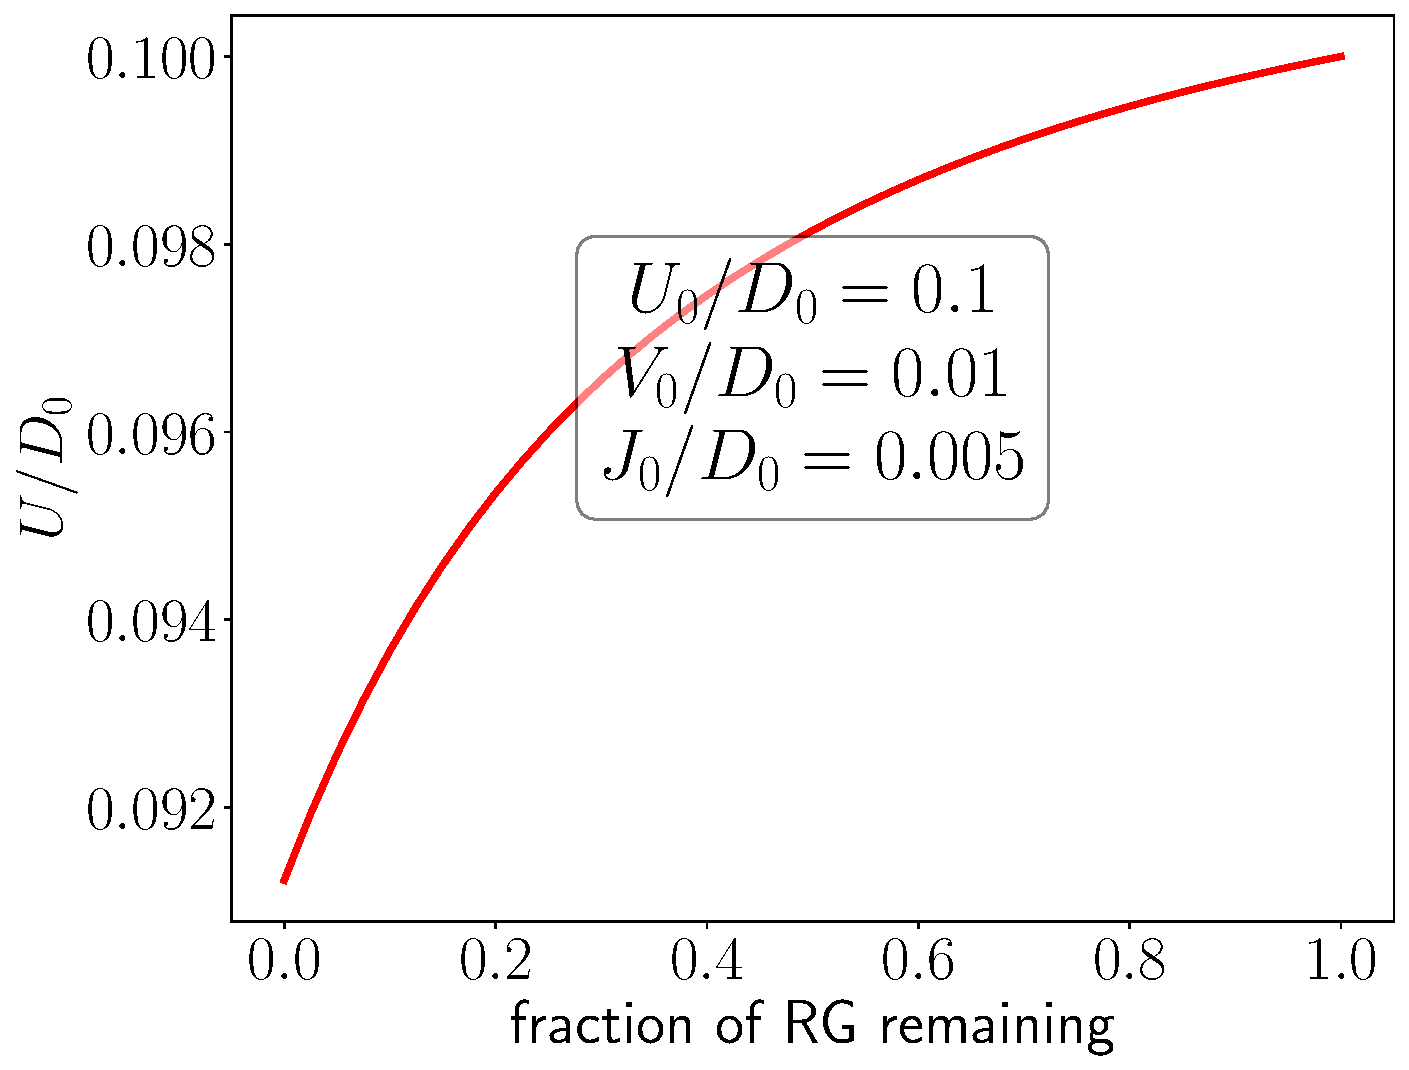
\includegraphics[width=0.32\textwidth]{../figures/U_irr,U>0,U.pdf}
	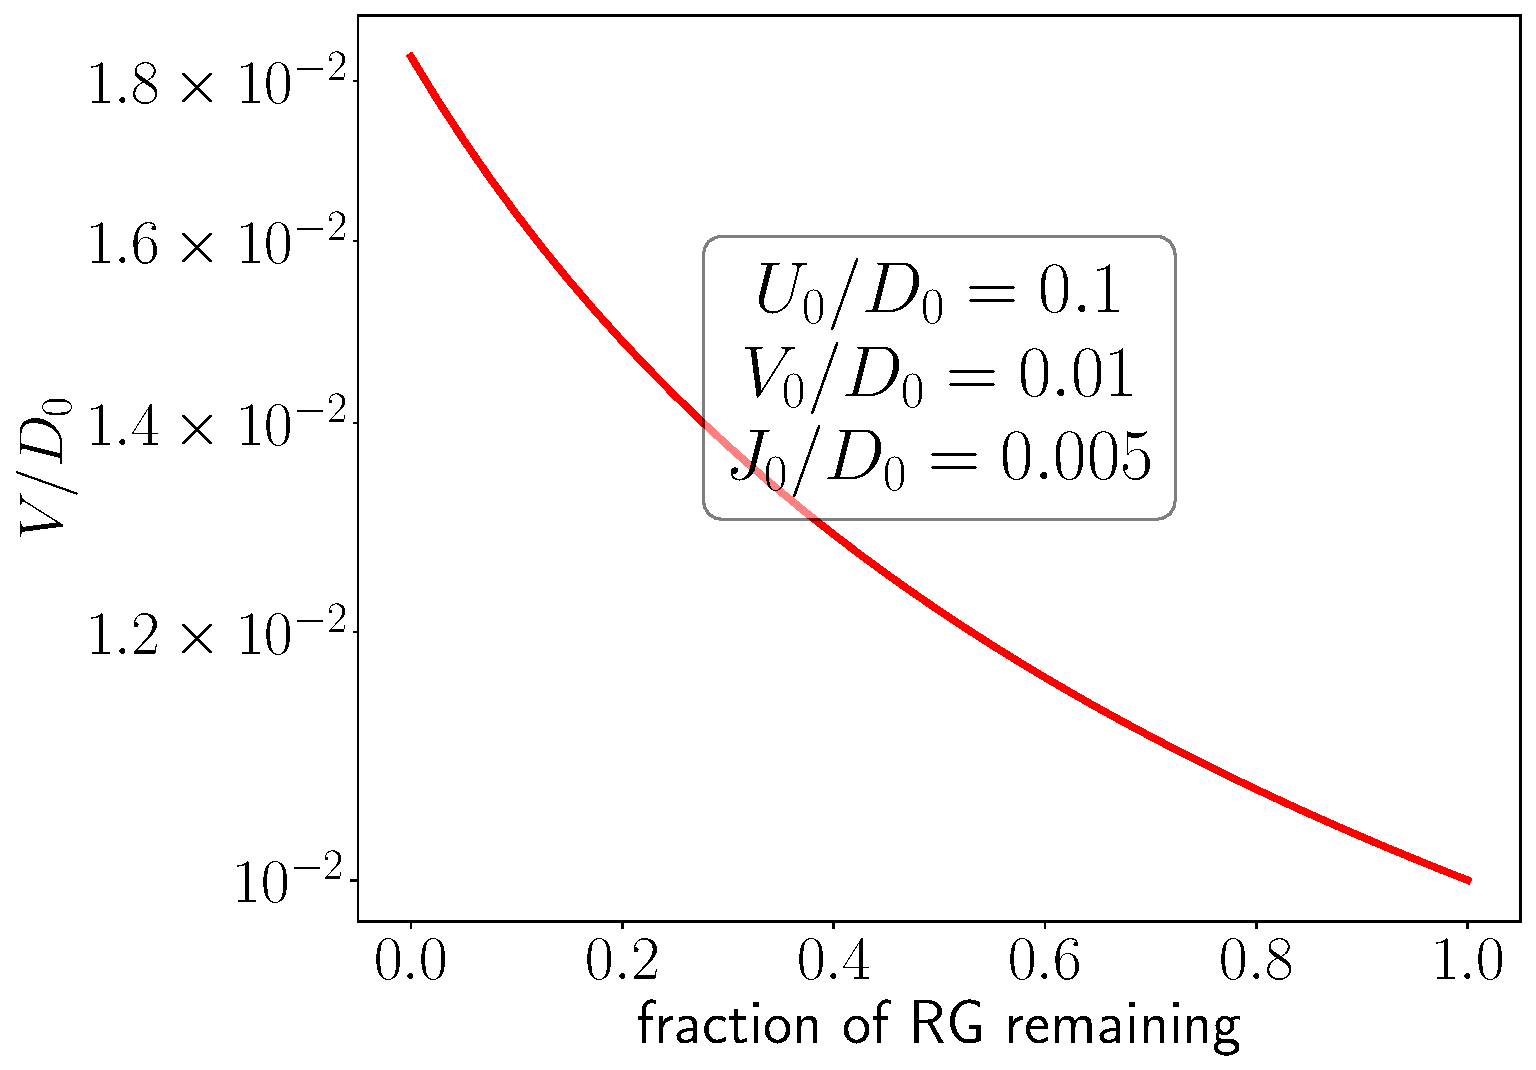
\includegraphics[width=0.32\textwidth]{../figures/U_irr,U>0,V.pdf}
	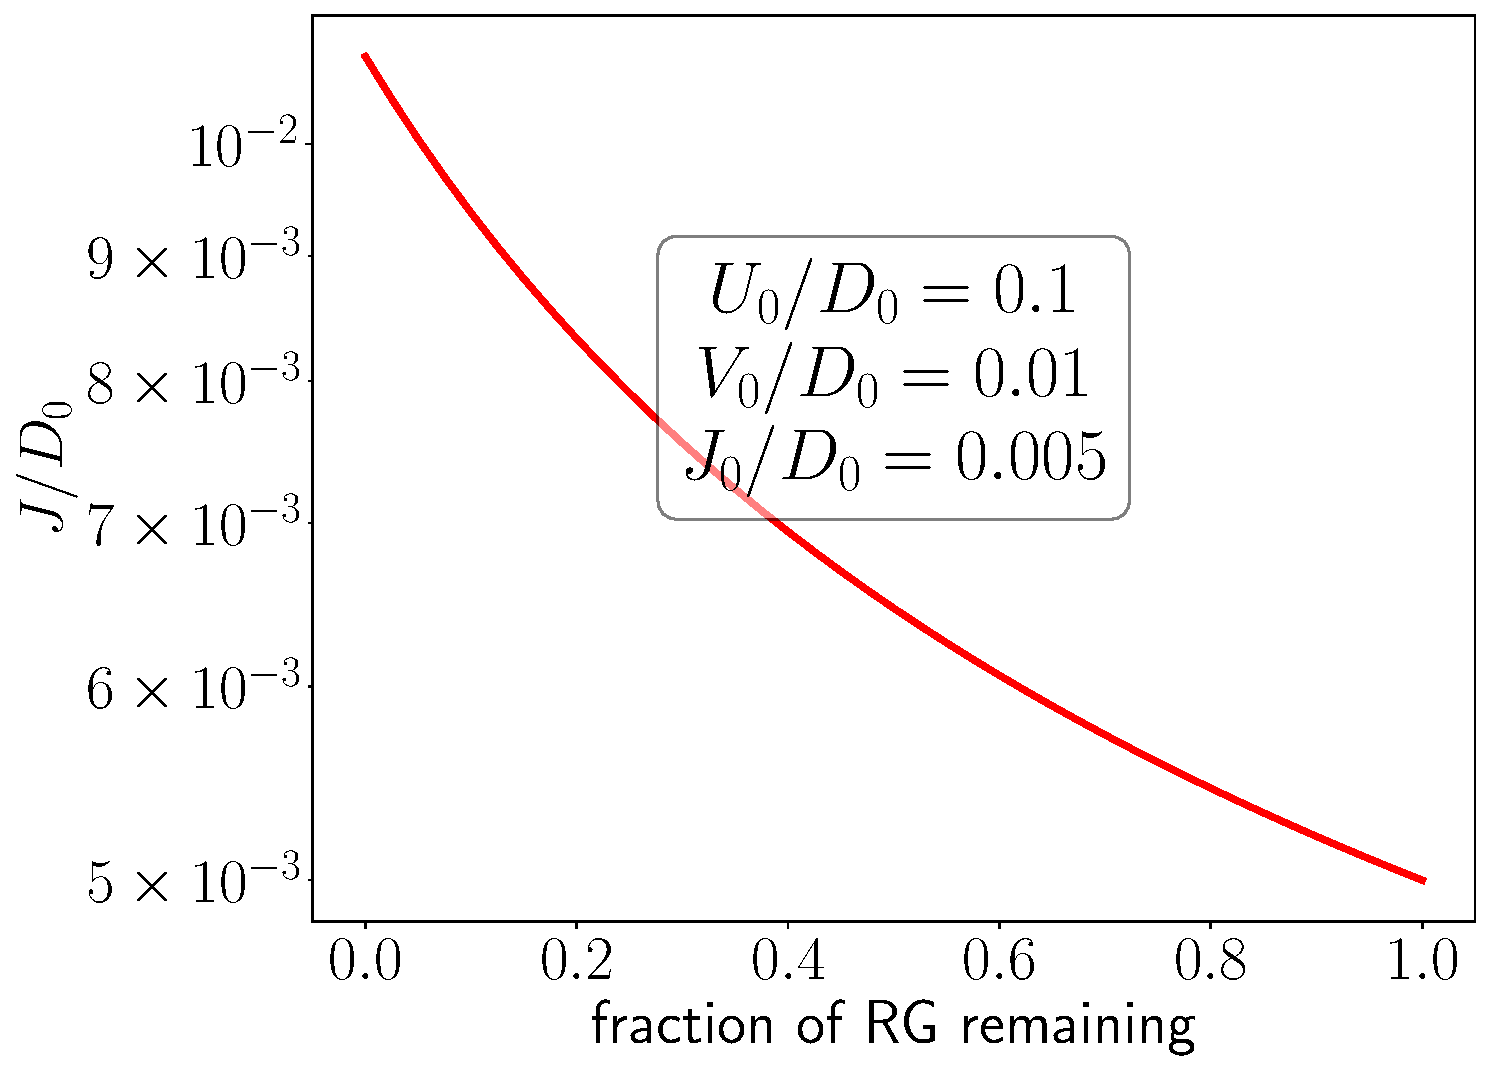
\includegraphics[width=0.32\textwidth]{../figures/U_irr,U>0,J.pdf}

	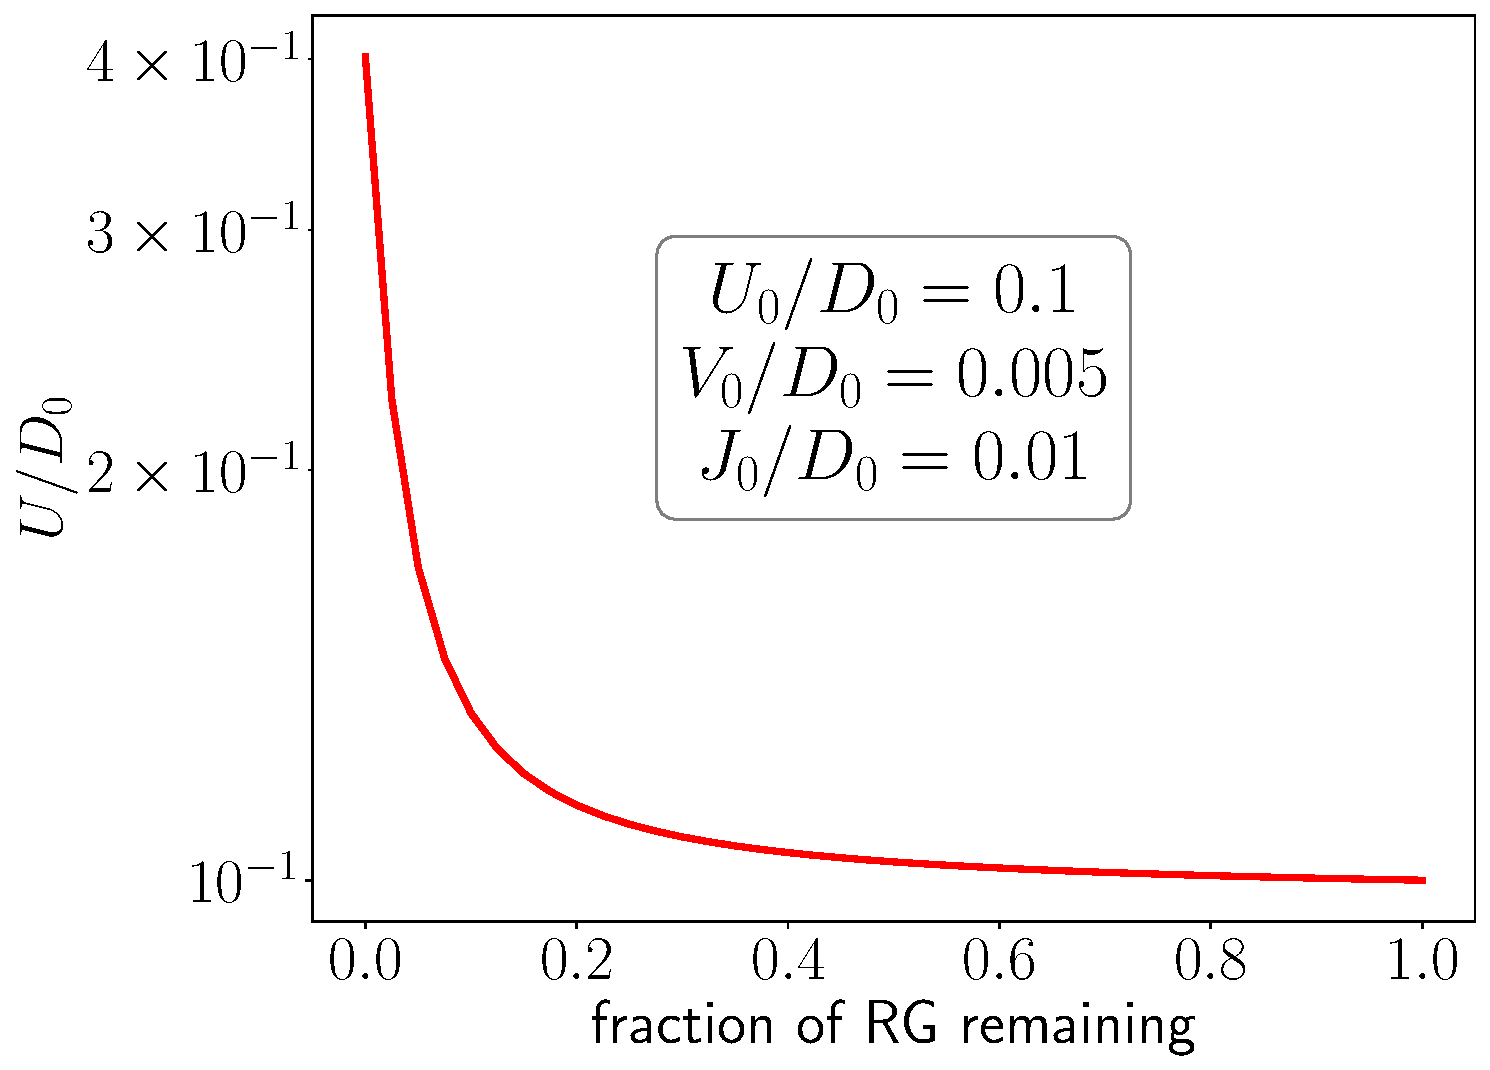
\includegraphics[width=0.32\textwidth]{../figures/U_rel,U>0,U.pdf}
	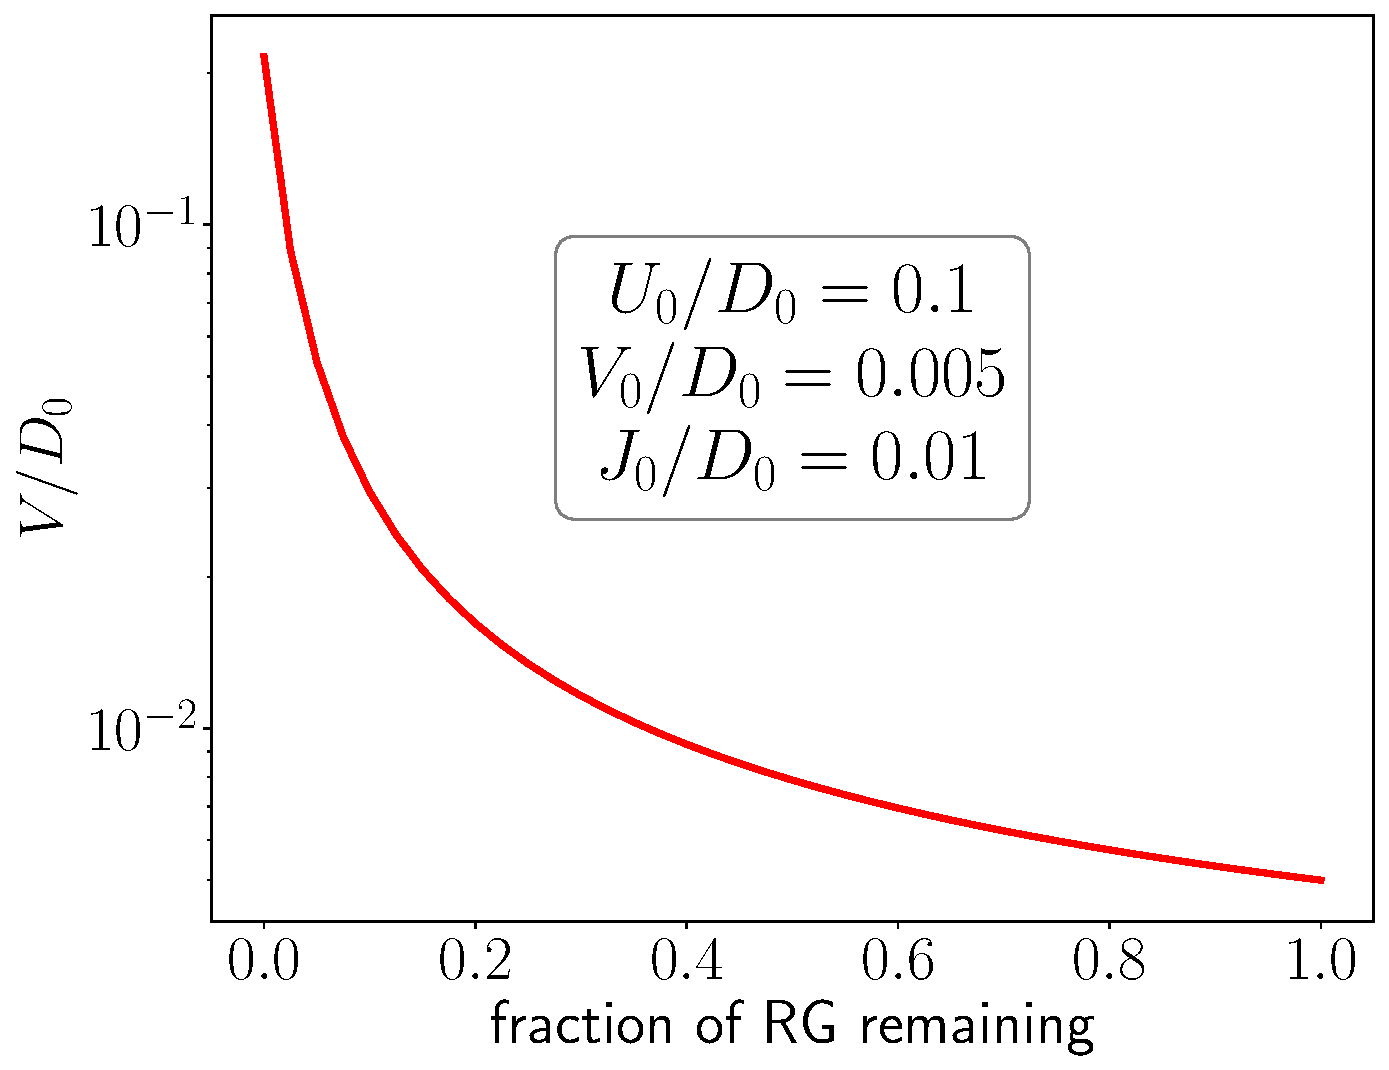
\includegraphics[width=0.32\textwidth]{../figures/U_rel,U>0,V.pdf}
	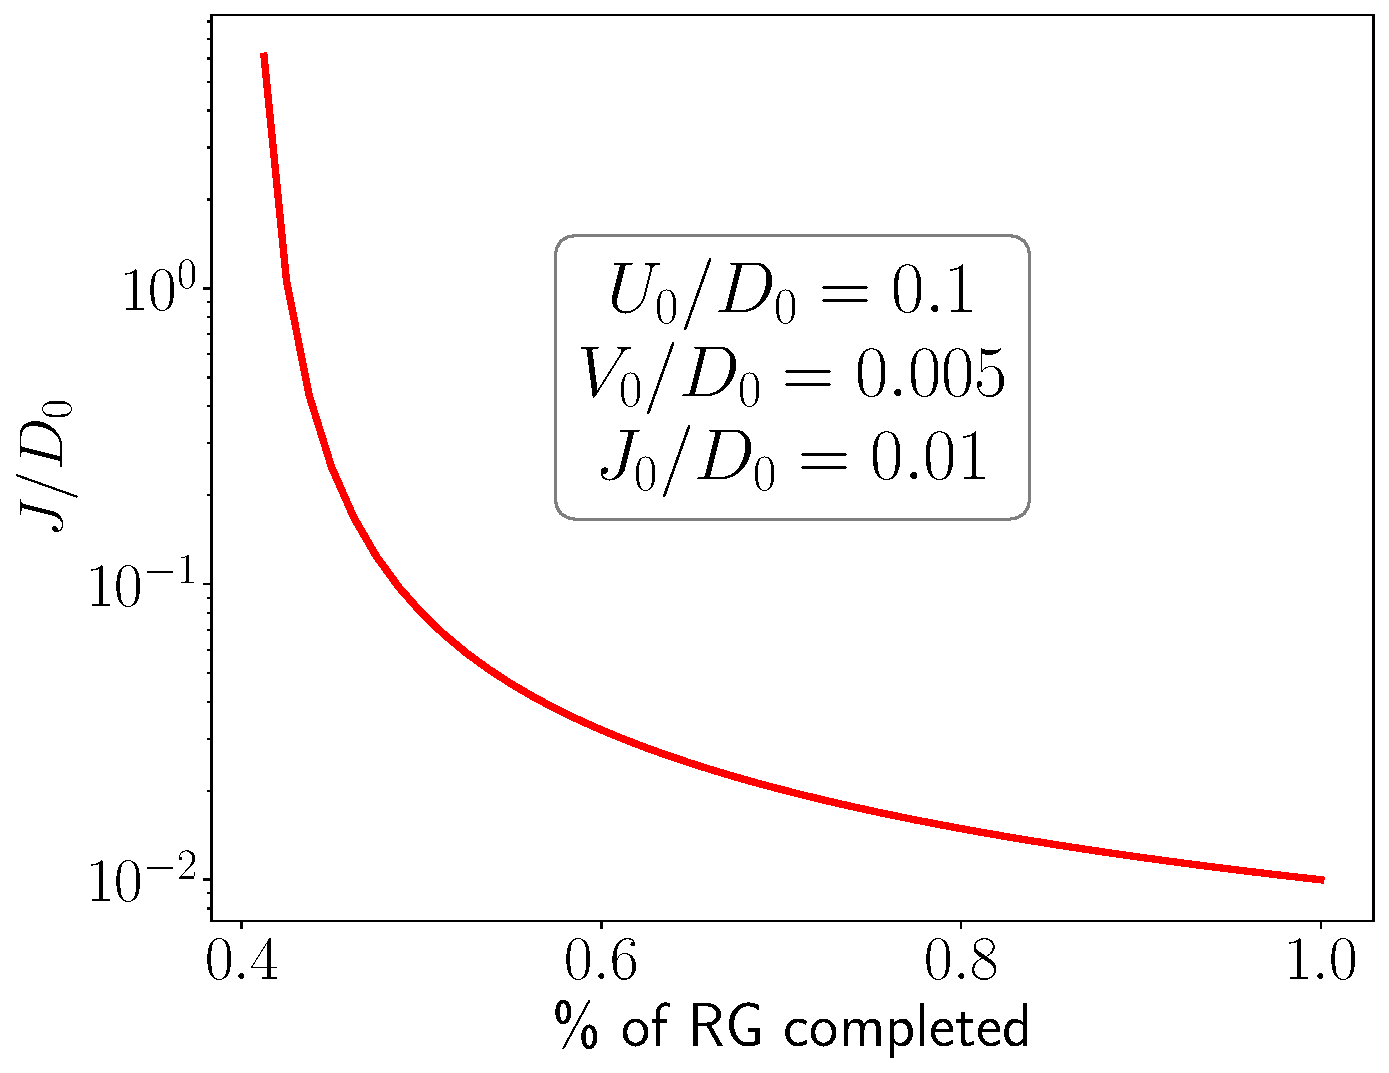
\includegraphics[width=0.32\textwidth]{../figures/U_rel,U>0,J.pdf}
\end{figure}

\begin{figure}[htpb]
	\centering
	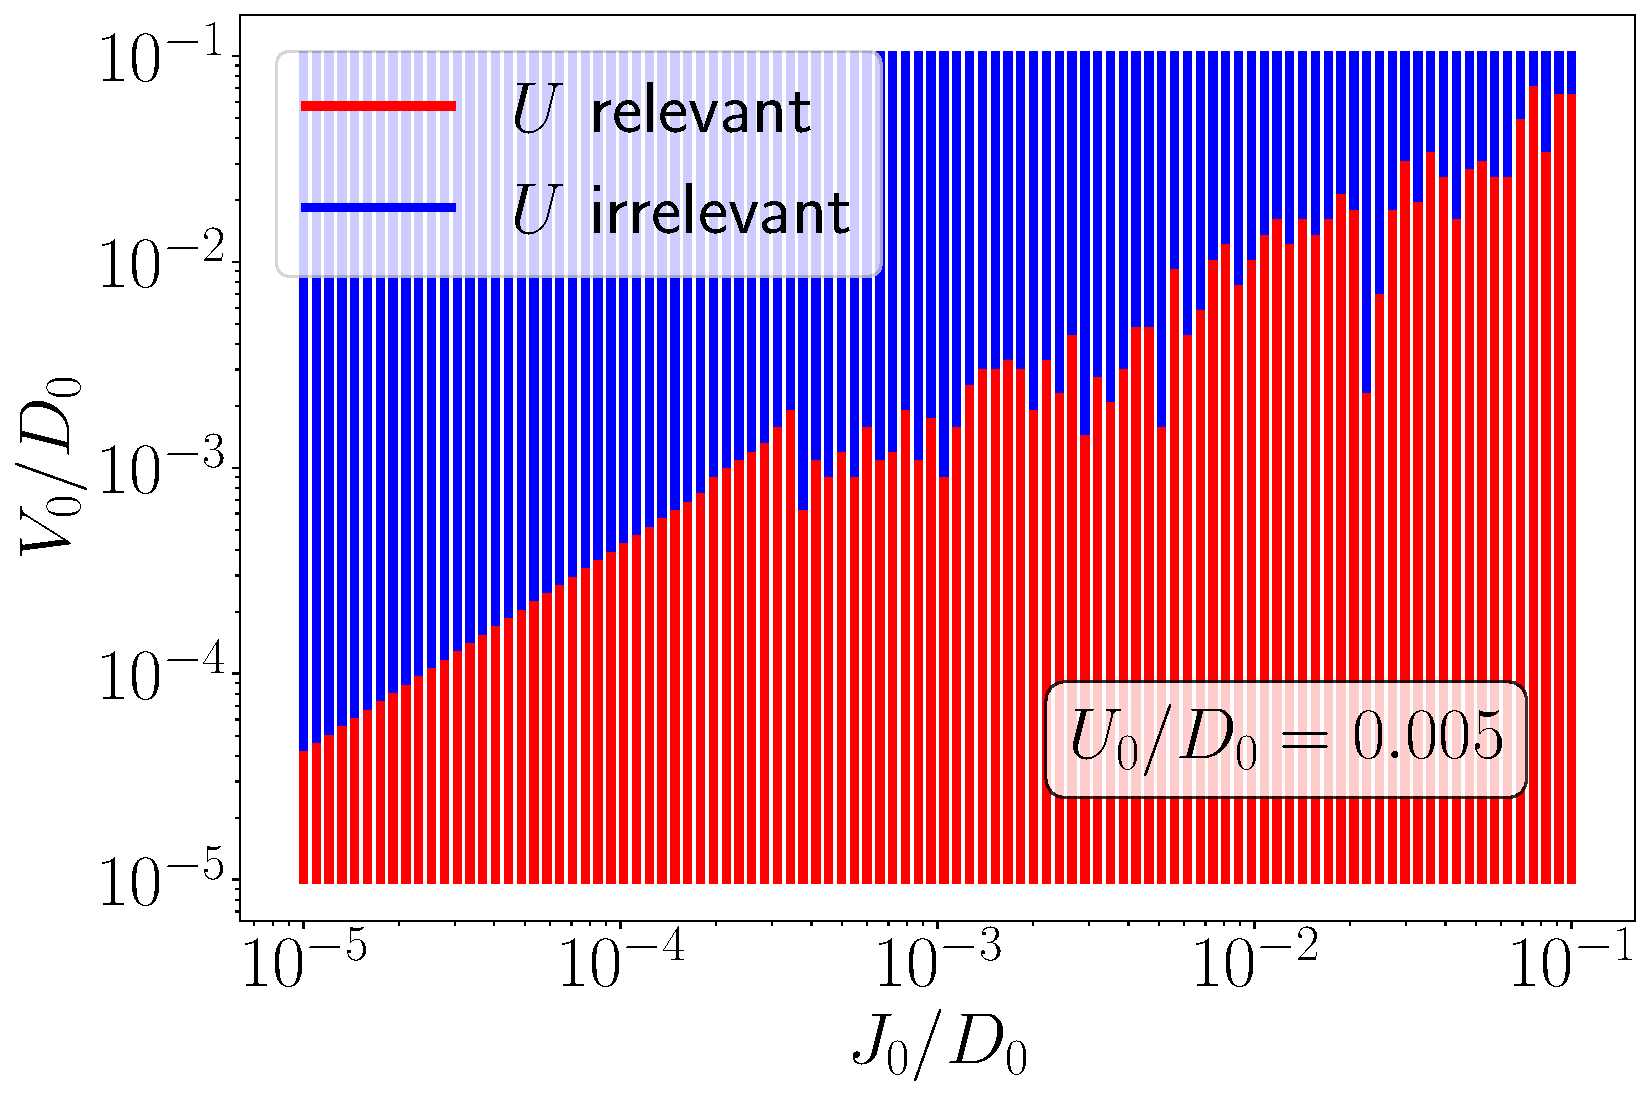
\includegraphics[width=0.48\textwidth]{../figures/VvsJ_relvsirr.pdf}
	\hspace*{\fill}
	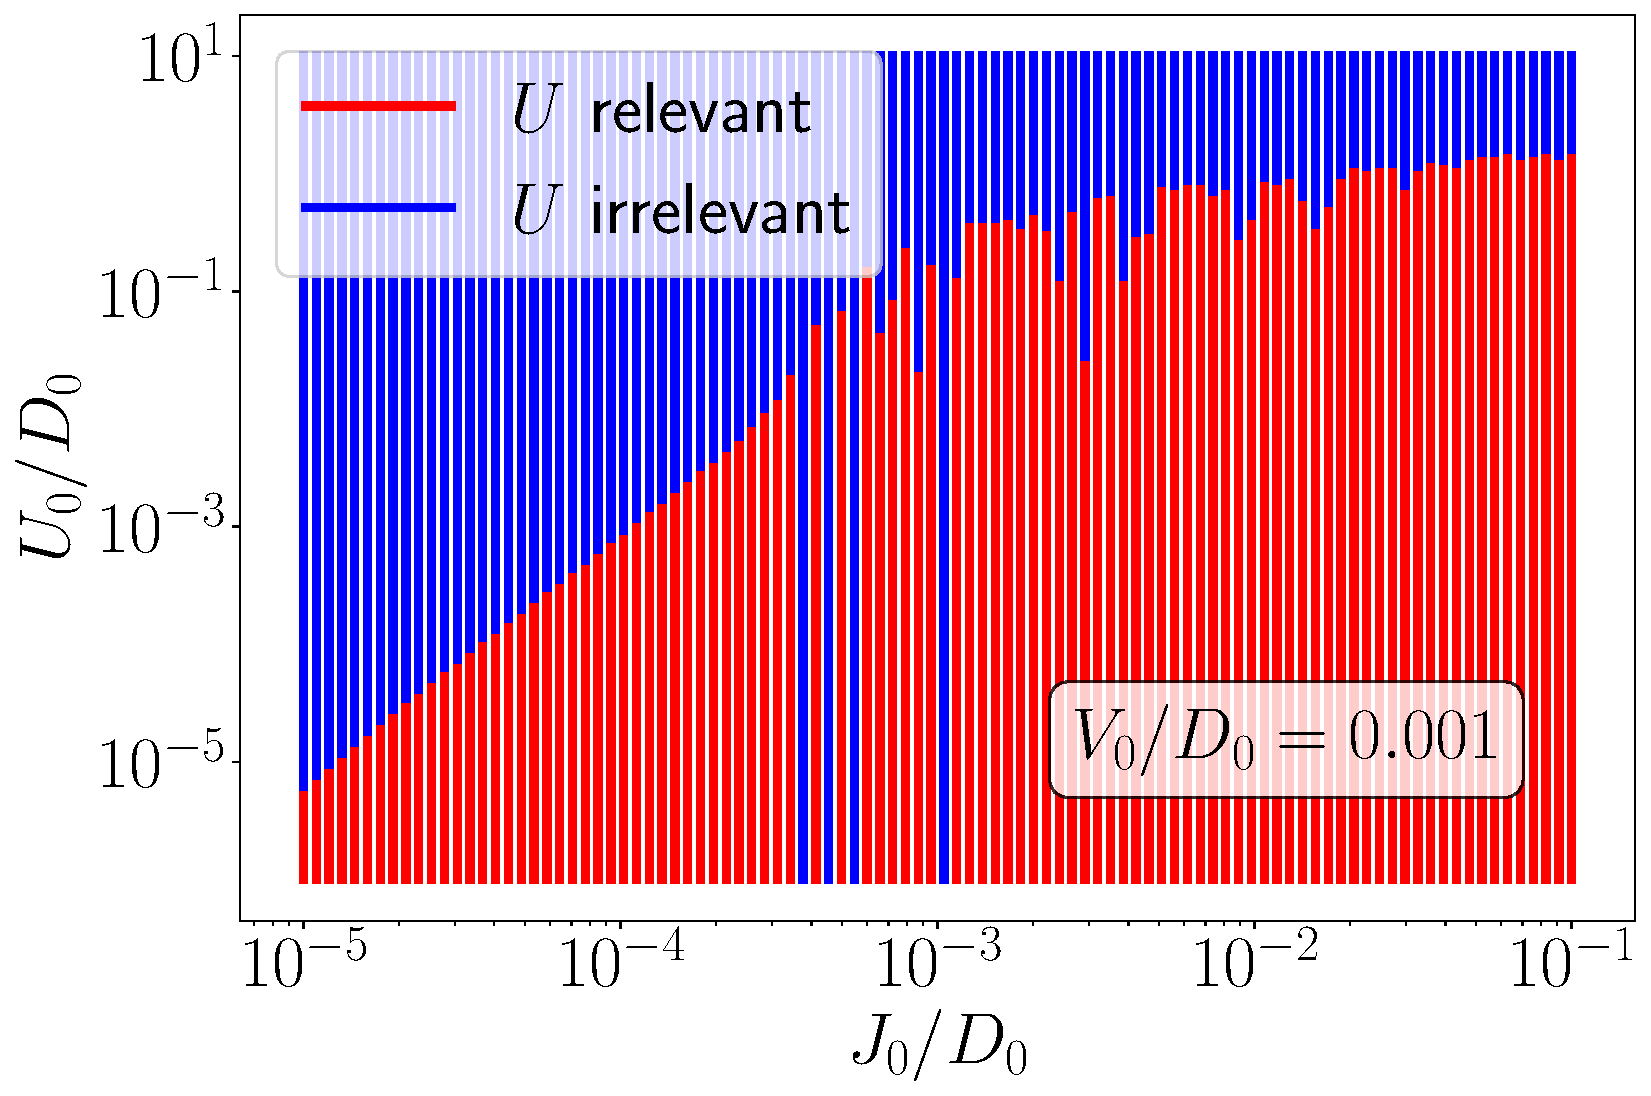
\includegraphics[width=0.48\textwidth]{../figures/UvsJ_relvsirr.pdf}
\end{figure}

\begin{figure}[htpb]
	\centering
	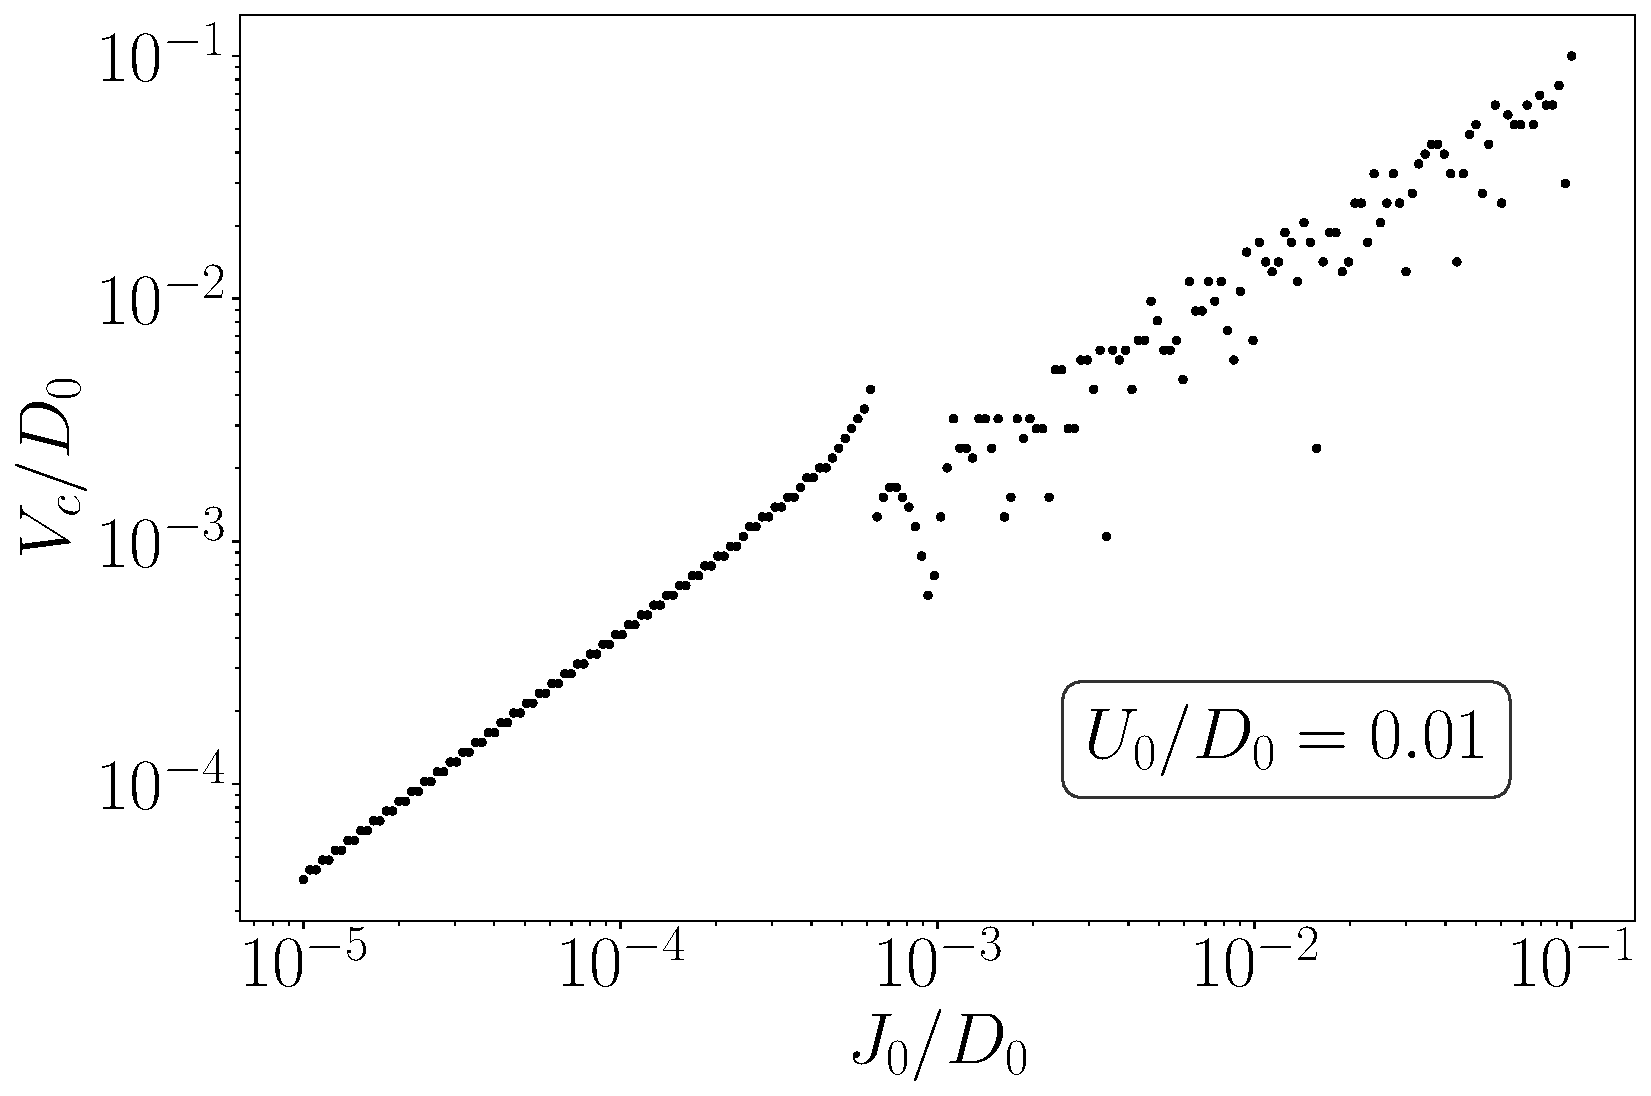
\includegraphics[width=0.48\textwidth]{../figures/VcvsJ.pdf}
	\hspace*{\fill}
	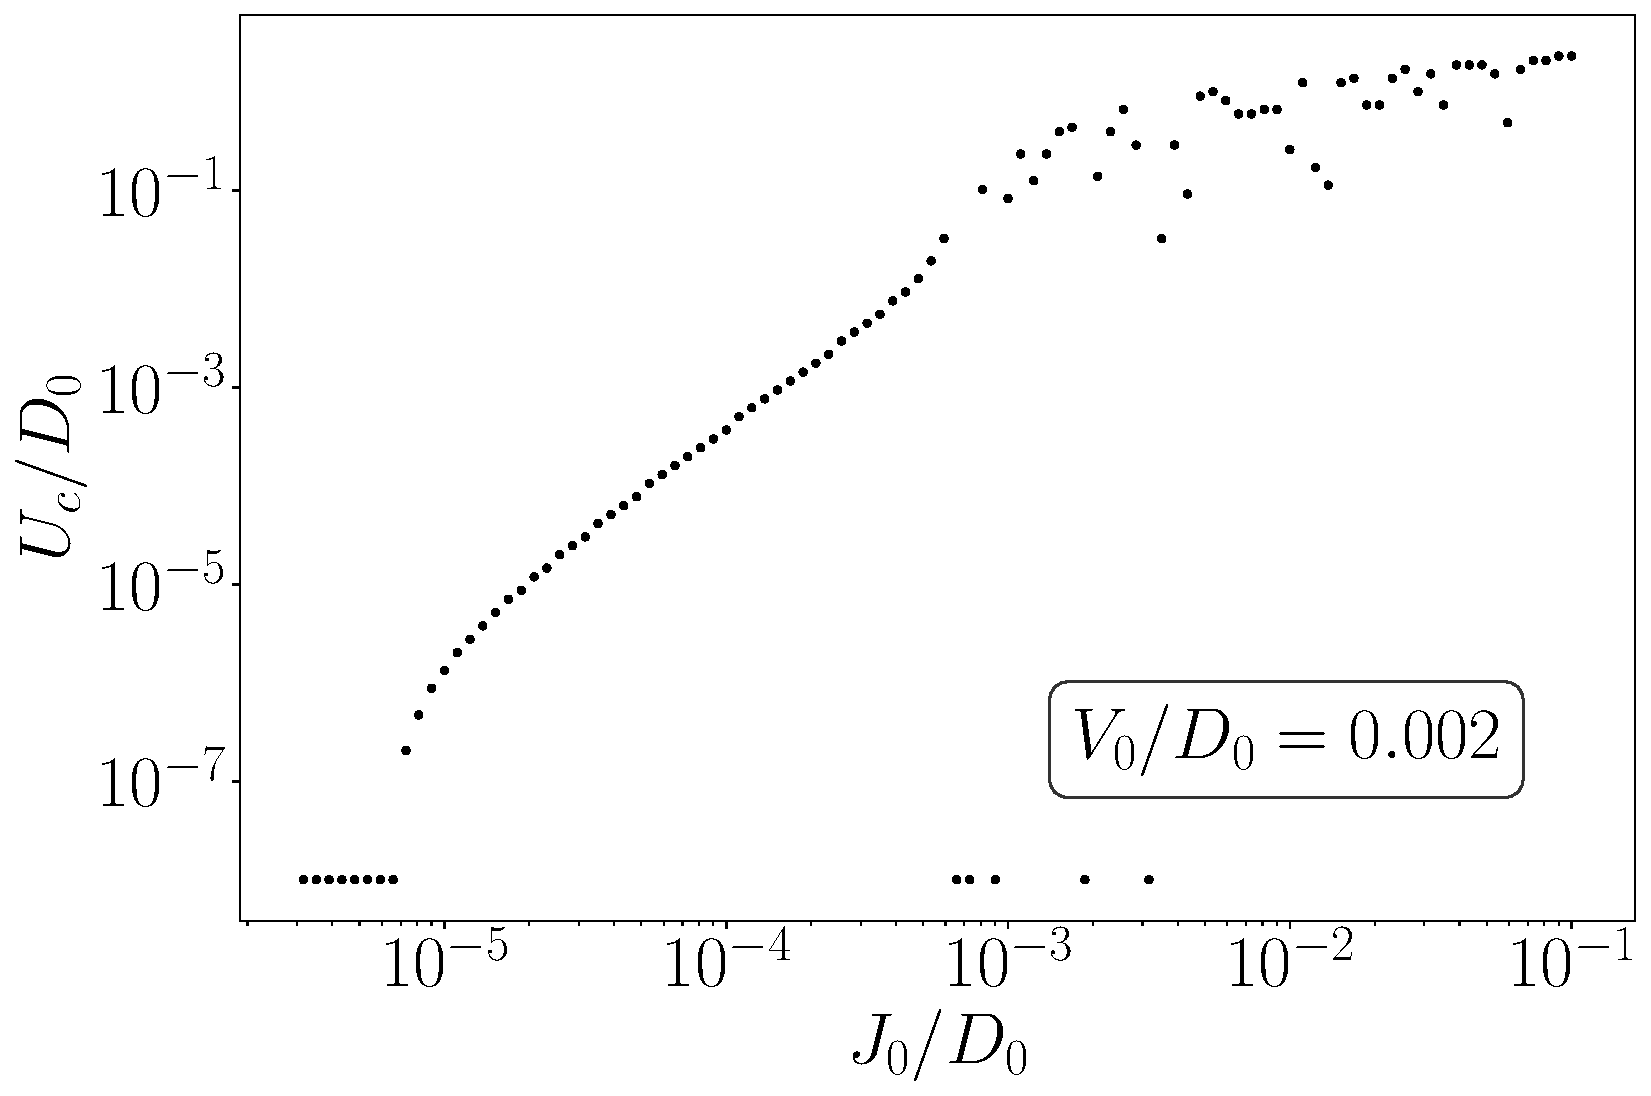
\includegraphics[width=0.48\textwidth]{../figures/UcvsJ.pdf}
	% \caption{../figures/UcvsJ.pdf}
	% \label{fig:-figures-UcvsJ-pdf}
\end{figure}

\subsection{Attractive interaction on impurity: \(U<0\)}
Here, we have \(J<0\) and \(K>0\). The denominators satisfy the following inequality in this regime:
\begin{equation}\begin{aligned}
	d_0 > d_3 > d_2 > d_1
\end{aligned}\end{equation}

The strong-coupling regime here corresponds to \(d_0 < 0\). This again means that all the denominators are negative. The spin-exchange coupling \(J\) is now irrelevant, because its bare value is negative while its RG equation is positive: \(\Delta J>0\). Moreover, the isospin coupling \(K\) is now positive and so is its RG equation: \(\Delta K>0\), which means it flows to strong-coupling. \(V\) also flows to strong-coupling. The RG equation for \(U\) can be written as
\begin{equation}\begin{aligned}
	\Delta U = 4V^2\left(\frac{K}{4} - U\right)\frac{n_j}{d_0 d_1} + \frac{n_j K^2}{d_3}
\end{aligned}\end{equation}
The first term is necessarily positive, while the second term is negative. This means that for roughly \(V_0 > J_0\), we  will have \(\Delta U > 0\), and since \(U_0 < 0\), this amounts to an irrelevant flow of \(U\) towards zero. On the other hand, for \(J_0 > V_0\), we will have \(\Delta U < 0\), and this corresponds to a relevant flow of \(U\) towards large negative value.

In other words, the RG flows in this regime can be exactly mapped to those in the positive \(U\) regime. The general statement is: in the strong-coupling regime of positive(negative) \(U\), \(V\) is always relevant, \(J\)(\(K\)) is relevant, \(K\)(\(J\)) is irrelevant, and \(U\) is relevant when \(J(K) > V\), otherwise \(U\) is irrelevant.


\section{Effective Hamiltonian and ground state}
The fixed point Hamiltonian can, in general, be written as
\begin{equation}\begin{aligned}
	\mathcal{H}^* = \sum_{\sigma, k}\epsilon_k \tau_{k\sigma} - \frac{U^*}{2}\left(\hat n_{d \uparrow} - \hat n_{d \downarrow}\right)^2  + \sum_{\sigma, k < \Lambda^*}\left( V^* c^\dagger_{k\sigma}c_{d\sigma} + \text{h.c.} \right) + J^* \vec{S_d}\cdot\vec{s} + K^* \vec{C_d}\cdot\vec{C}
\end{aligned}\end{equation}
The first term is the kinetic energy of all the electrons. The next two terms are the impurity-diagonal pieces, featuring the renormalised interaction \(U^*\). The next three terms are the residual interactions between the impurity and the metal, with the renormalised couplings \(V^*, J^*\) and \(K^*\). The summations in these terms extend from the fixed point momentum cutoff \(\Lambda^*\) to 0. This is the region of momentum space  which the URG was unable to decouple. The operators \(\vec s\) and \(\vec C\) represent the macroscopic magnetic and charge spins formed by the remaining electrons that are lying inside the window \(\left[ 0, \Lambda^* \right] \):
\begin{equation}\begin{aligned}
	\vec s = \sum_{kk^\prime<\Lambda^*\atop{\alpha\beta}} c^\dagger_{k\alpha}\vec \sigma_{\alpha\beta}c_{k^\prime\beta}
\end{aligned}\end{equation}
Our goal here is to write down the ground state wavefunction for this low-energy Hamiltonian.

To make progress, we will simplify the effective Hamiltonian by taking the zero bandwidth limit. This reduces it to a two-site problem. One site is of course the impurity site, and this site will be labeled as site 1. The other site will be formed by the center of mass degree of freedom of the conduction electrons, and will be labeled as site 2. The Hamiltonian for this two-site problem is
\begin{equation}\begin{aligned}
	\mathcal{H}_{IR} = - \frac{U^*}{2}\left(\hat n_{1 \uparrow} - \hat n_{1 \downarrow}\right)^2 + V^*\sum_{\sigma}\left(c^\dagger_{1\sigma}c_{2\sigma} + \text{h.c.} \right) + J^*\vec{S_1}\cdot\vec{S_2} + K^* \vec{C_1}\cdot\vec{C_2}
\end{aligned}\end{equation}
\begin{figure}[!htb]
	\centering
	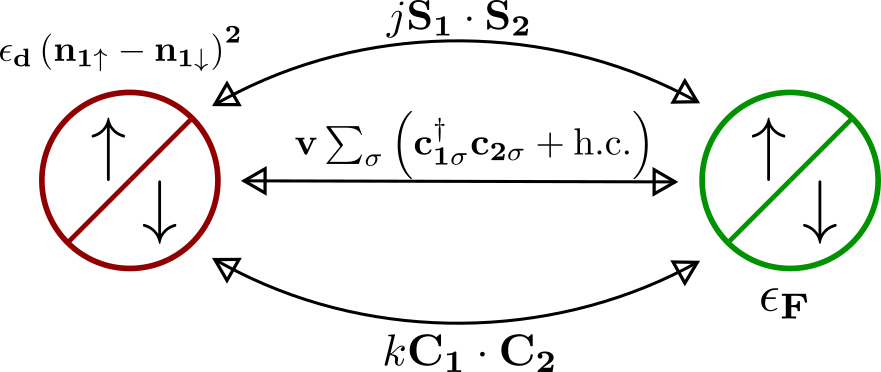
\includegraphics[width=0.4\textwidth]{../figures/two_site_problem.png}
	\caption{Two-site effective problem of fixed point Hamiltonian}
	\label{twosite}

\end{figure}
The subscripts on the operators designate the site on which they act; \(\hat n_1\) is the number operator for the first site.

We will adopt the following notation to represent the states in this Hilbert space. A general state will be represented in the Fock space basis as \(\ket{n_{1 \uparrow}n_{1 \downarrow}n_{2 \uparrow}n_{2 \downarrow}}\). For example,
\begin{equation}\begin{aligned}
	\ket{1101} = c^\dagger_{1 \uparrow}c^\dagger_{1 \downarrow}c^\dagger_{2 \downarrow}\ket{-}
\end{aligned}\end{equation}
\(\ket{-}\) is the vacuum state.

% The full list of eigenstates is given in Table~\ref{twosite_spectrum}.
% \begin{table}[htb!]
% 	\centering
% 	\begin{tabular}{|c|c|c|c|}
% 		\hline
% 		\(\hat n\) & \(S_1^z + S_2^z\) & eigenstate & eigenvalue\\
% 		\hline
% 		0 & 0 & \(\ket{0,0}\) & \(\frac{1}{4}{K^*}\)\\
% 		\hline
% 		4 & 0 & \(\ket{2,2}\) & \(\frac{1}{4}{K^*}\)\\
% 		\hline
% 		\multirow{2}{*}{1} & \(\frac{1}{2}\) & \(-4{V^*}\ket{\uparrow,0} +2 \left[-\frac{1}{2}U^* \mp \Delta\left(U^* , {V^*}\right)\right] \ket{0, \uparrow}\) & \multirow{2}{*}{\(-\frac{1}{4}U^* \pm \frac{1}{2}\Delta\left(U^* , {V^*}\right)\)}\\
% 		 & - \(\frac{1}{2}\) & \(-4{V^*}\ket{\downarrow,0} +2 \left[-\frac{1}{2}U^* \mp \Delta\left(U^* , {V^*}\right)\right] \ket{0, \downarrow}\)  &\\
% 		\hline
% 		\multirow{2}{*}{3} & \(\frac{1}{2}\) & \(-4{V^*}\ket{\uparrow,2} +2 \left[-\frac{1}{2}U^* \mp \Delta\left(U^* , {V^*}\right)\right] \ket{2, \uparrow}\) & \multirow{2}{*}{\(-\frac{1}{4}U^* \pm \frac{1}{2}\Delta\left(U^* , {V^*}\right)\)}\\
% 		 & - \(\frac{1}{2}\) & \(-4{V^*}\ket{\downarrow,2} +2 \left[-\frac{1}{2}U^* \mp \Delta\left(U^* , {V^*}\right)\right] \ket{2, \downarrow}\)  &\\
% 		\hline
% 		\multirow{3}{*}{2} & 1,-1,0 & \(\ket{\uparrow,\uparrow}\), \(\ket{\downarrow,\downarrow}\), \(\ket{\uparrow,\downarrow} + \ket{\downarrow, \uparrow}\) & {\(-\frac{1}{2}U^* + \frac{1}{4}{J^*}\)}\\
% 		\cline{2-4}
% 		& 0 & \(\ket{2,0} - \ket{0,2}\) & \(-\frac{3}{4}{K^*}\)\\
% 		\cline{2-4}
% 		& 0 & \(c_\pm^s \frac{1}{\sqrt 2}\left(\ket{\uparrow, \downarrow} - \ket{\downarrow, \uparrow}\right) + c^c_\pm \frac{1}{\sqrt 2}\left(\ket{\uparrow\downarrow, 0} + \ket{0, \uparrow\downarrow}\right)\) & \({V^*}\left[ \gamma \pm \sqrt{\gamma^2 + 4} \right] -\frac{1}{2}U^* - \frac{3}{4}{J^*}\)\\
% 		\hline
% 	\end{tabular}
% 	\caption{Eigenstates for effective two-site Hamiltonian}
% 	\label{twosite_spectrum}
% \end{table}
% The quantities \(\Delta\) and \(\gamma\) are defined as
% \begin{equation}\begin{aligned}
% 	\label{gamma_def}
% 	\Delta\left(U^*, V^*\right) = \frac{1}{2}\sqrt{{U^*}^2 + 16{V^*}^2}, \quad \gamma = \frac{1}{2{V^*}}\left[ \frac{1}{4}\left( 3J^* + K^* \right) + \frac{1}{2}U^* \right] 
% \end{aligned}\end{equation}

For \(U>0\), the ground state is given by
\begin{gather}
	\label{gstate}
	\ket{\Psi}_\text{1} = c_s \frac{1}{\sqrt 2}\left(\ket{\uparrow, \downarrow} - \ket{\downarrow, \uparrow}\right) + c_c \frac{1}{\sqrt 2}\left(\ket{\uparrow\downarrow, 0} + \ket{0, \uparrow\downarrow}\right), \quad E_1 =  -V^*\sqrt{\gamma^2 + 4} -\frac{1}{4}U^* - \frac{3}{8}{J^*}
\end{gather}
where $\gamma = \frac{1}{2{V^*}}\left[ \frac{1}{4}\left( 3J^* + K^* \right) + \frac{1}{2}U^* \right]$. The probabilities for the spin and charge sectors for the ground state are
\begin{equation}\begin{aligned}
	\label{coeff_def}
	\left(c_s\right)^2 = \frac{1}{2\sqrt{\gamma^2 + 4}}\left(\sqrt{\gamma^2 + 4} + \gamma\right), \quad \left(c_c \right)^2 = \frac{1}{2\sqrt{\gamma^2 + 4}}\left(\sqrt{\gamma^2 + 4} - \gamma\right)~.
\end{aligned}\end{equation}
For (roughly) \(J_0 > V_0\), we get \(J^* \gg V^*\) and \(U^* \gg U_0\) so that \(\gamma \gg 1\). This gives \(\left( c_s \right) ^2 \sim 1\) and \(\left( c_c \right) ^2 \sim 0\). The entire contribution to the ground state then comes from the spin sectors of the two sites. This is calculated numerically in fig.~\ref{cs_cc}.
\begin{figure}[htpb]
	\centering
	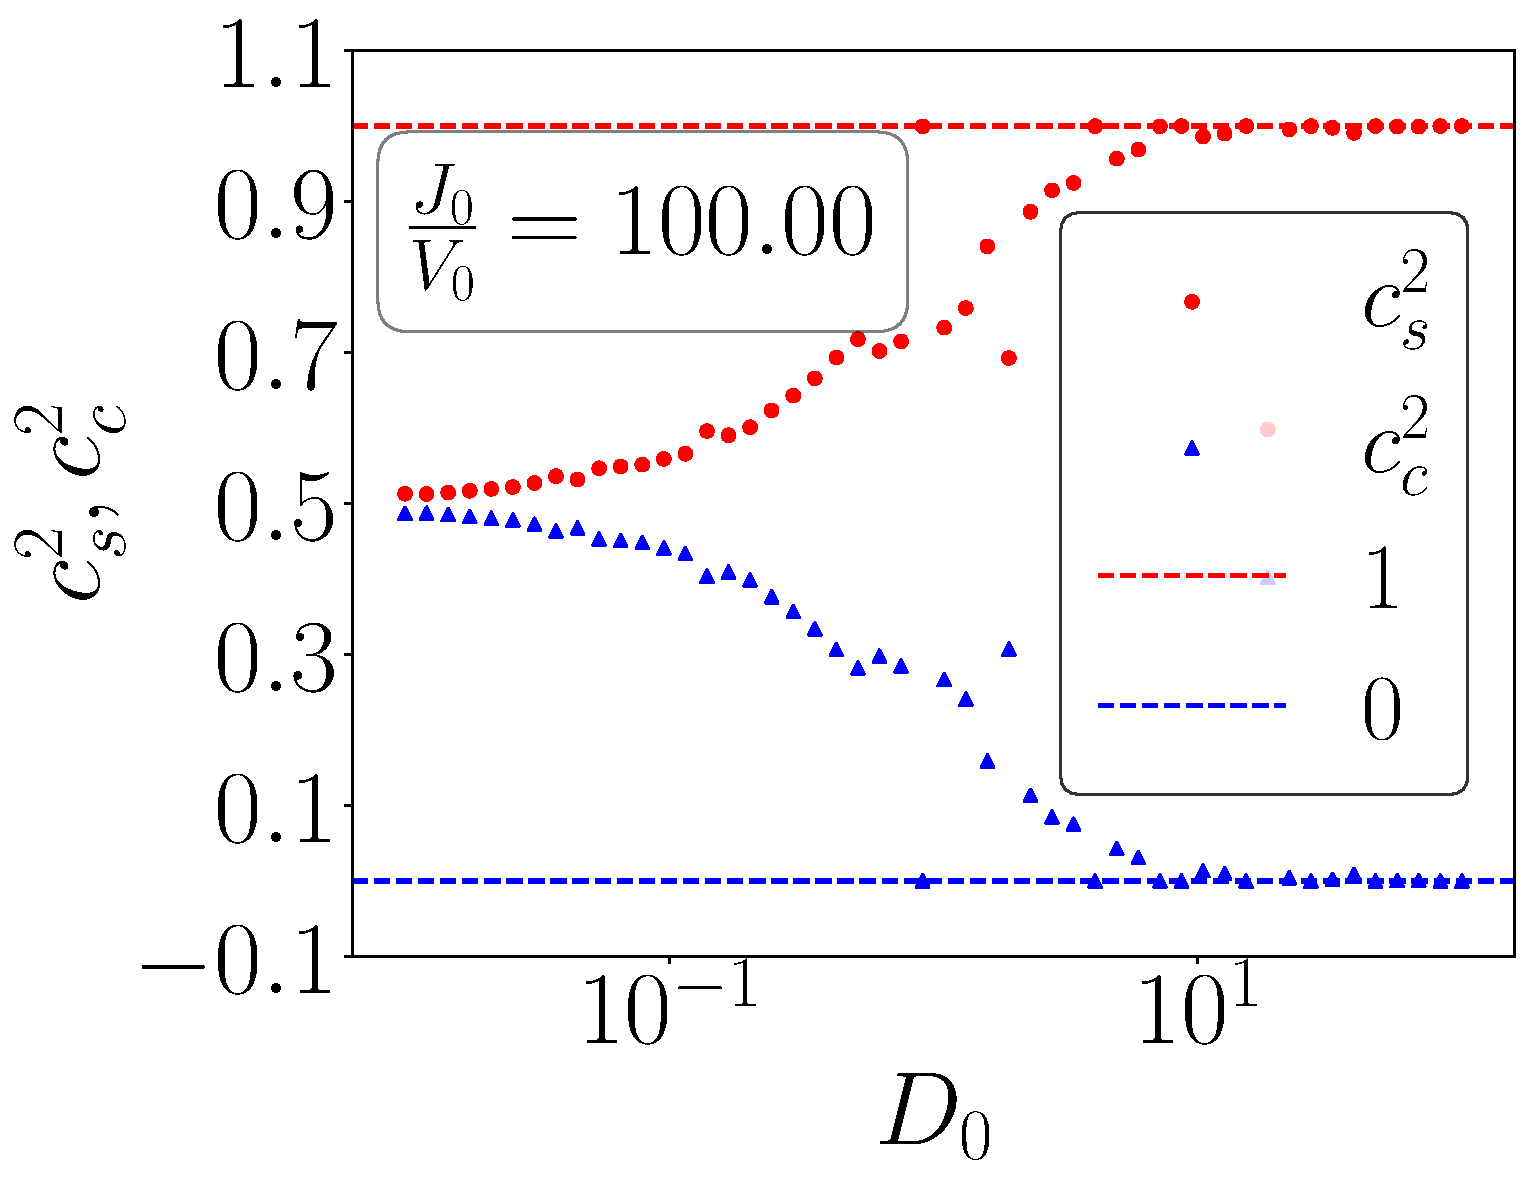
\includegraphics[width=0.8\textwidth]{../figures/coeffs_vs_J.pdf}
	\caption{Variation of relative weights \(c_s\) and \(c_c\) with \(J_0\)}
	\label{cs_cc}
\end{figure}

In the other regime of \(U<0\), the two competing states are \(\ket{\Psi}_1\) defined above (with energy \(E_1\)), and \(\ket{\Psi_2}\), the charge singlet: \(\ket{\Psi}_2 = \frac{1}{\sqrt 2}\left( \ket{2,0} - \ket{0,2} \right)\) having energy \(E_2\).
\begin{equation}\begin{aligned}
	E_2 = -\frac{3}{4}K^*, \quad E_1 - E_2 = -\frac{1}{4}\sqrt{\left( \frac{1}{2}K^* + U^* \right)^2 + (4V^*)^2} - \frac{1}{4}U^* + \frac{3}{4}K^*
\end{aligned}\end{equation}
For \(V_0 \gg K_0\), the largest energy scale will be \(V^*\), and we can then approximate this difference as
\begin{equation}\begin{aligned}
	E_1 - E_2 \simeq -V^* < 0
\end{aligned}\end{equation}
In such a case, \(\ket{\Psi}_1\) will therefore be the ground state. In the other regime \(V_0 \ll K_0\), the largest energy scale will be \(K^*\), and we can then write
\begin{equation}\begin{aligned}
	E_1 - E_2 \simeq - \frac{1}{8}K^* + \frac{3}{4}K^* > 0
\end{aligned}\end{equation}
In this case, the ground state will be \(\ket{\Psi}_2\). There exists, therefore, a phase transition at a critical plane \((U_c, K_c, V_c)\), where the ground state changes between the charge singlet \(\ket{\Psi}_2\) and the spin singlet + charge triplet \(\ket{\Psi}_1\).

\section{Approach towards the thermodynamic limit}
The URG method works strictly on finite systems and leads to finite values of fixed point couplings. The behaviour of the Hamiltonian in the thermodynamic limit can then be determined using finite-size scaling where we increase the bandwidth and decrease the width of each RG step. When applied to the fixed point value of the impurity-bath hybridisation parameter \(V\) (fig.~\ref{V_vs_D}), it can be seen that the fixed point value increases as the system size is increased, implying that the continuum limit of \(V^*\) is \(\infty\). This holds for both \(V_0 > J_0\) and \(V_0 < J_0\), as shown in the two panels of fig.~\ref{V_vs_D}.
\begin{figure}[htpb]
	\centering
	\hspace*{\fill}
	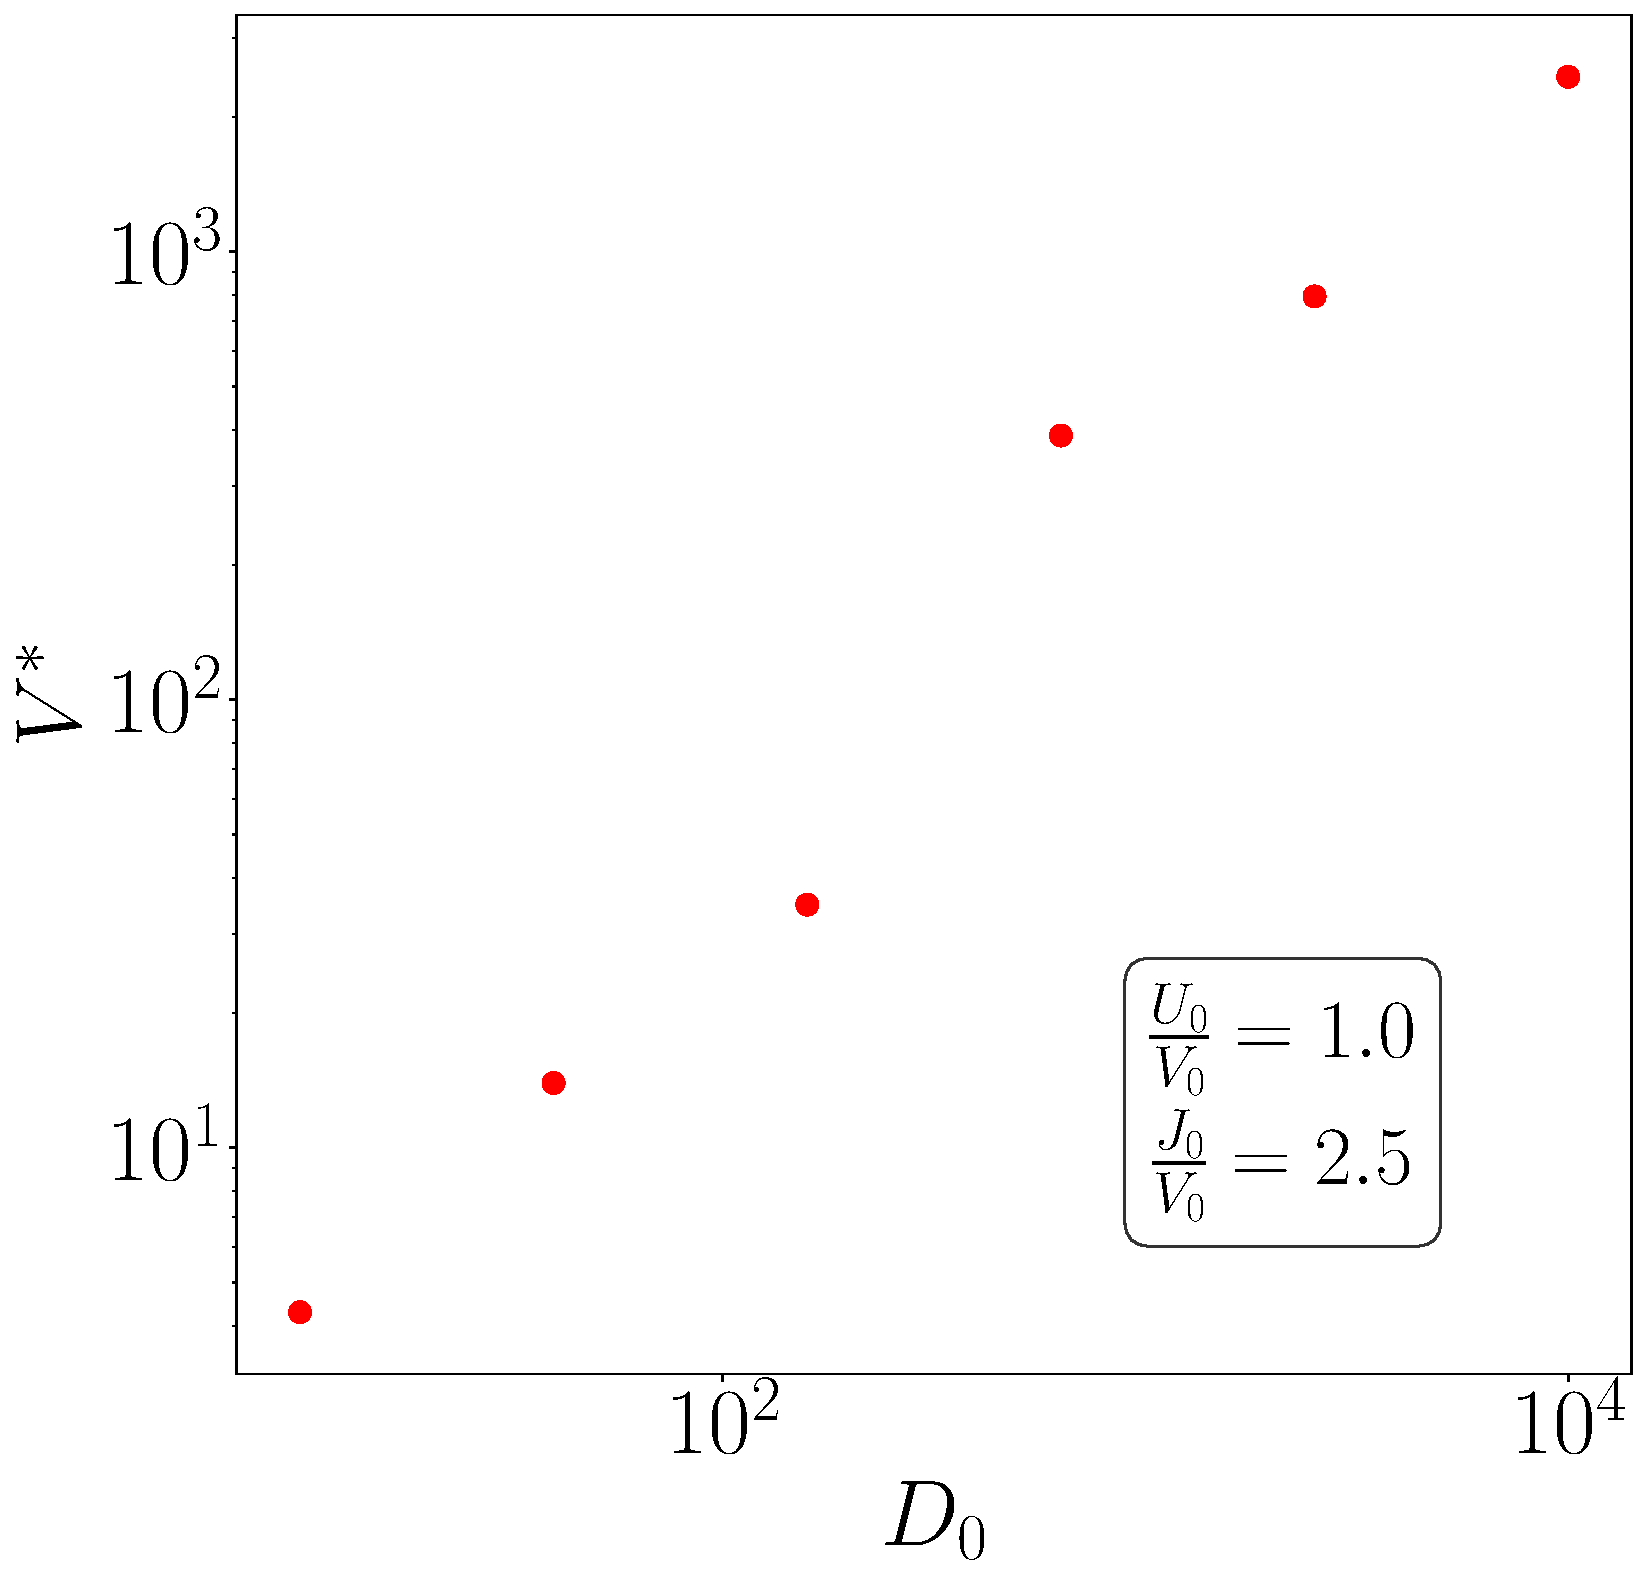
\includegraphics[width=0.4\textwidth]{../figures/Vstar_vs_D_smallV.pdf}
	\hspace*{\fill}
	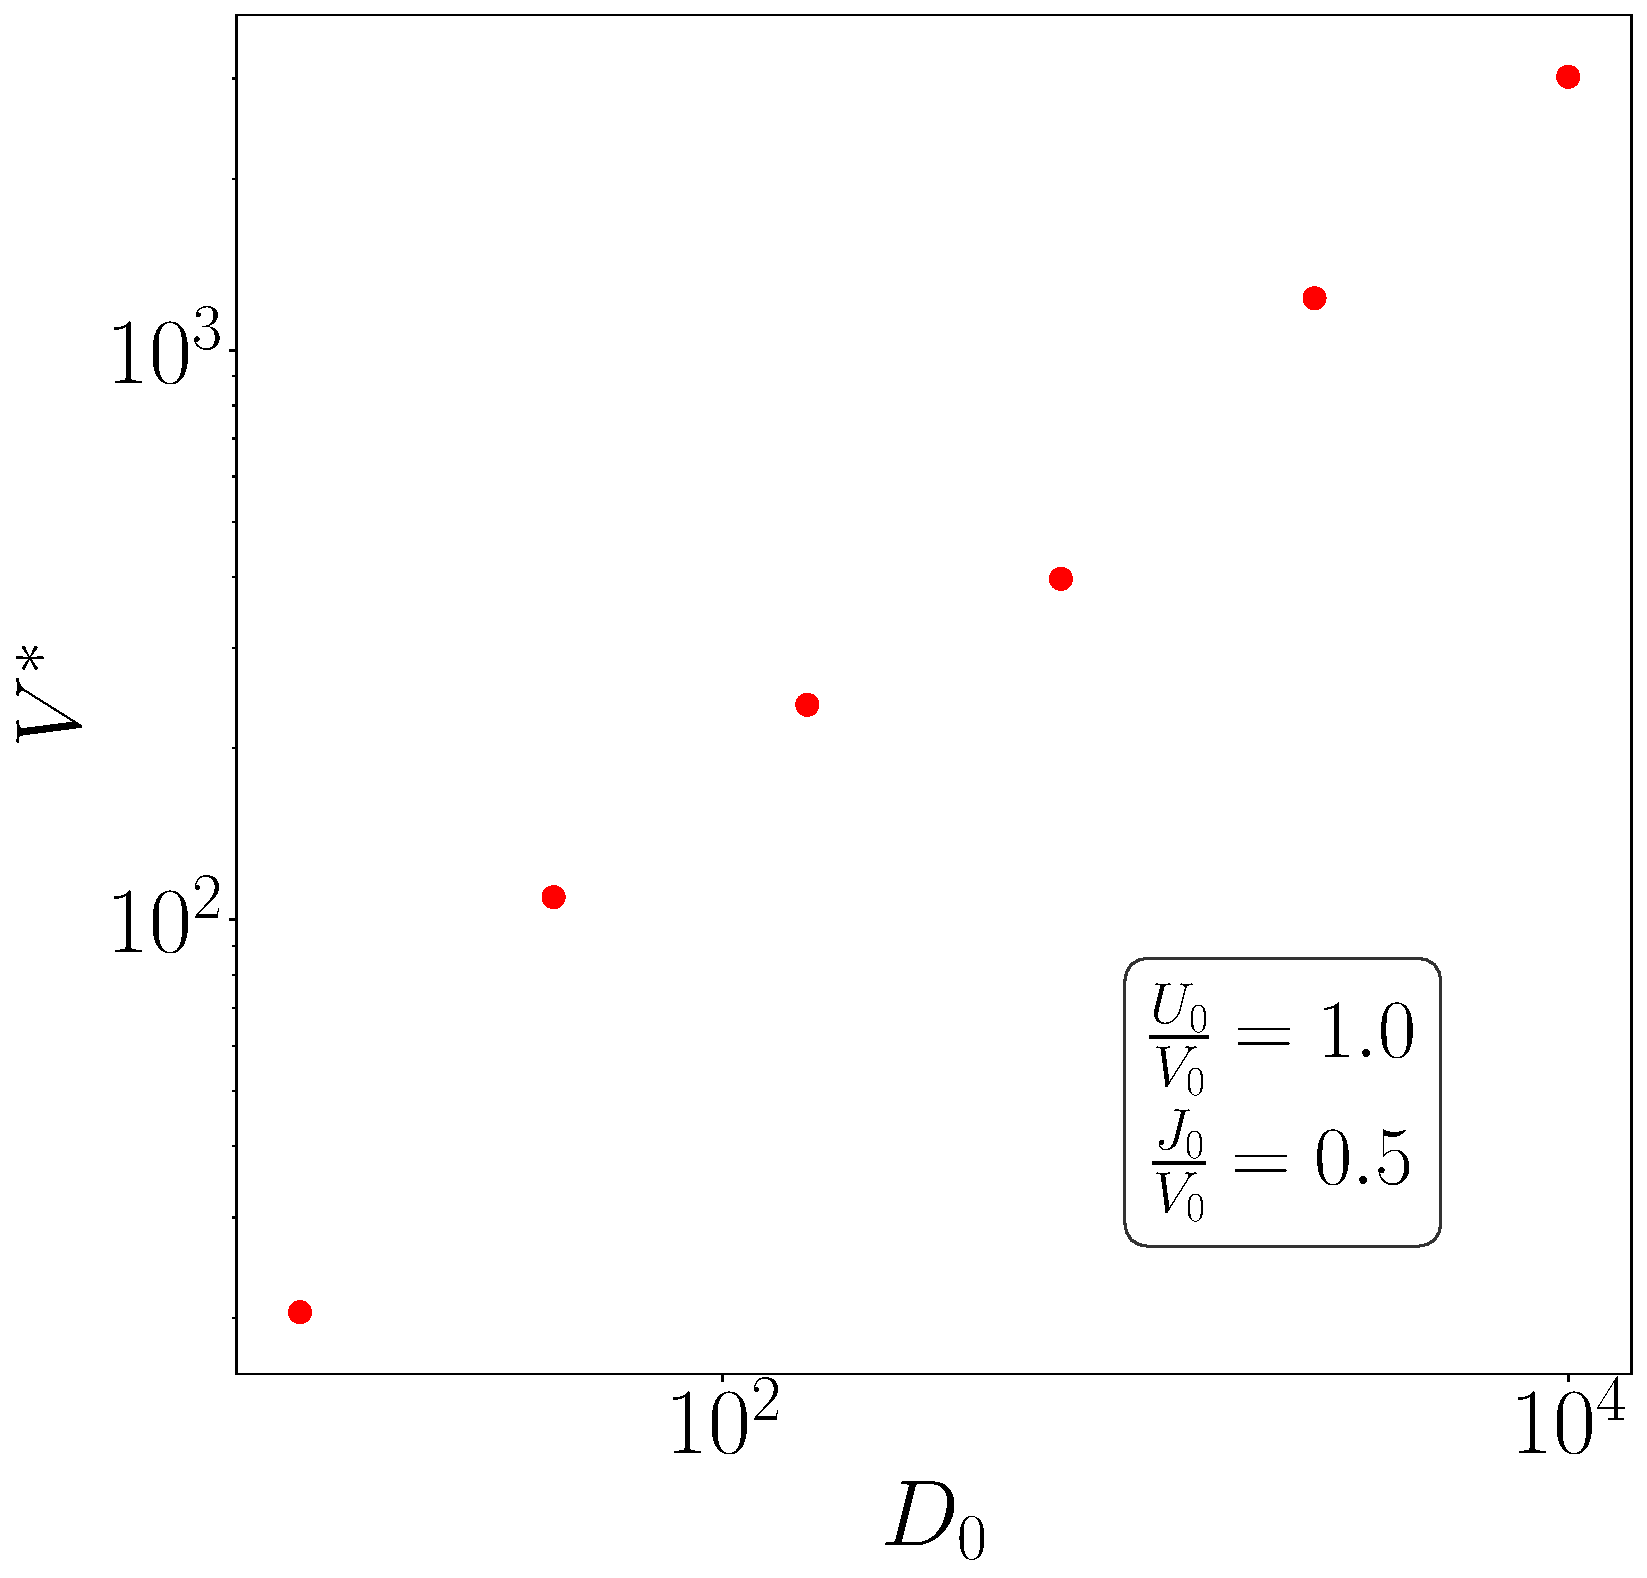
\includegraphics[width=0.4\textwidth]{../figures/Vstar_vs_D_largeV.pdf}
	\hspace*{\fill}
	\caption{Variation of fixed point value \(V^*\) with increasing bandwith \(D_0\), for both \(V_0 > J_0\) and \(V_0 < J_0\).}
	\label{V_vs_D}
\end{figure}

In a similar manner, we checked the variation of the spin and charge probabilities, \(c_s\) and \(c_c\), in the ground state, with increasing bandwith. The result is shown in fig.~\ref{c_vs_D}.
\begin{figure}[htpb]
	\centering
	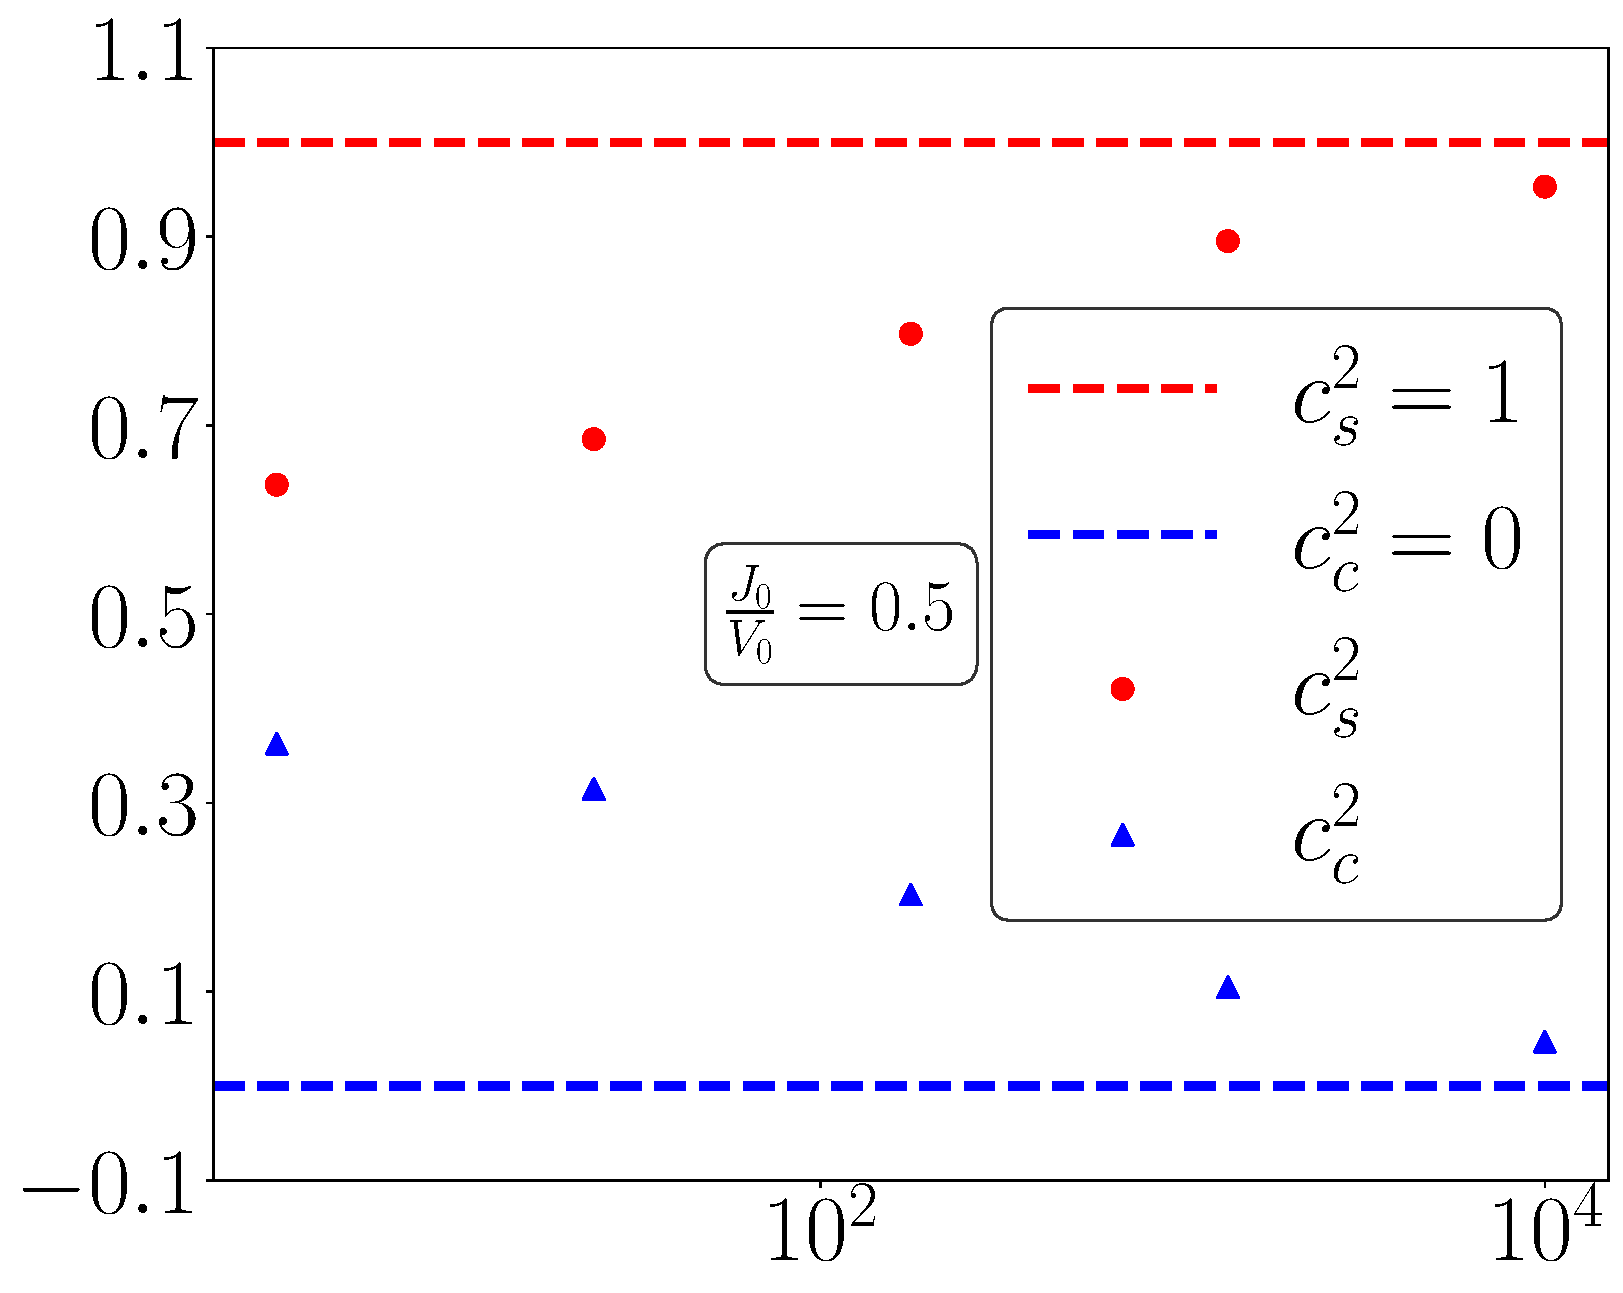
\includegraphics[width=0.45\textwidth]{../figures/coeffs_vs_D_largeV.pdf}
	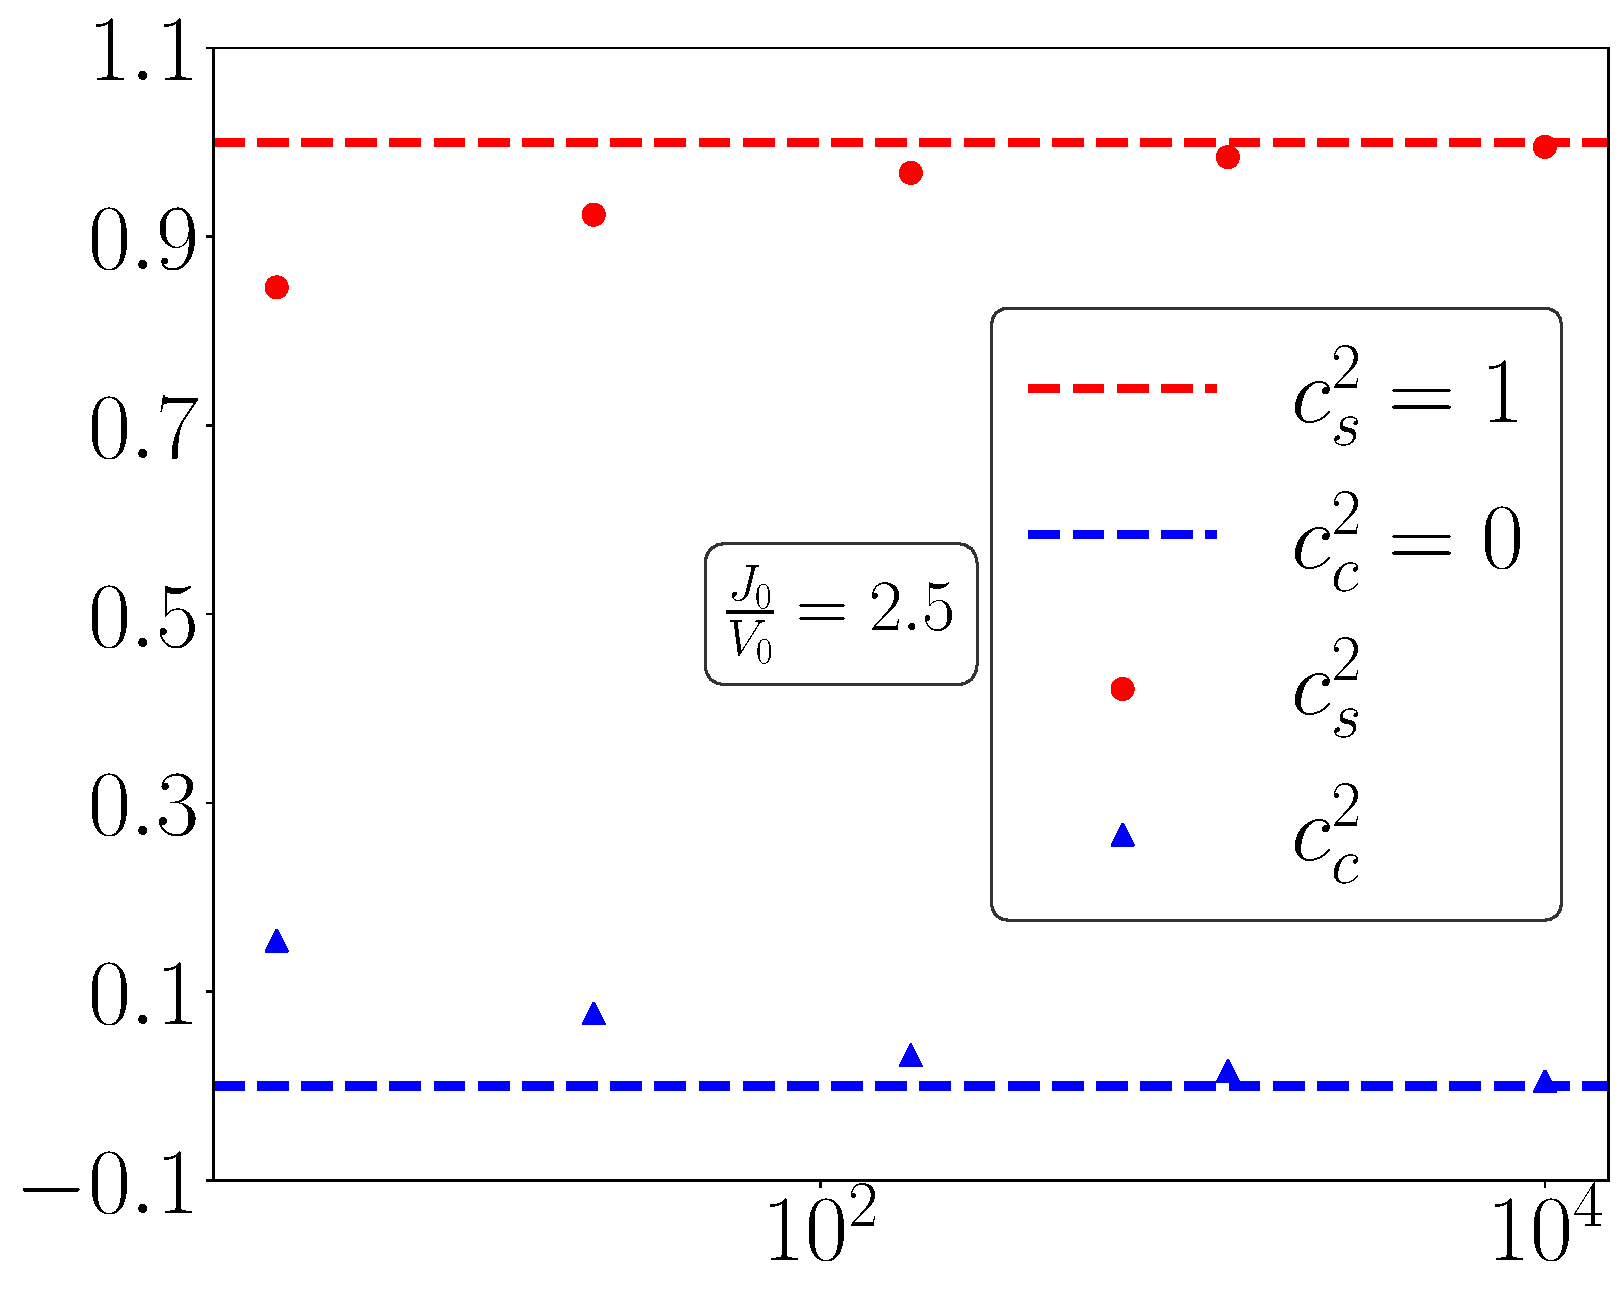
\includegraphics[width=0.45\textwidth]{../figures/coeffs_vs_D_smallV.pdf}
	\caption{Variation of spin and charge fractions, \(c_s\) and \(c_c\), of the ground state, as a function of bare bandwidth \(D_0\). Left and right panels show the cases of \(J_0 < V_0\) and \(J_0 > V_0\) respectively.}
	\label{c_vs_D}
\end{figure}
For both \(V_0 < J_0\) and \(V_0 > J_0\), we see that the spin contribution increases towards unity while the charge contribution vanishes. This indicates that at large bandwidth, the ground state becomes purely a spin singlet, formed purely by singly-occupied impurity states.
\begin{equation}\begin{aligned}
	\label{gstate_kondo}
	\lim_{D_0 \to \infty} \ket{\Psi}_1 = \frac{1}{\sqrt 2}\left(\ket{\uparrow, \downarrow} - \ket{\downarrow, \uparrow}\right) 
\end{aligned}\end{equation}
